\documentclass[a4paper, openany]{memoir}

\usepackage[utf8]{inputenc}
\usepackage[T1]{fontenc} 
\usepackage[english]{babel}

\usepackage{fancyhdr}
\usepackage{float}
\usepackage{graphics}
\usepackage{amsmath}
\usepackage{amsthm}
\usepackage{amssymb}
\usepackage{enumitem}
\usepackage{multicol}
\usepackage[bookmarksopen=true,bookmarksopenlevel=2]{hyperref}
\usepackage{tikz}
\usepackage{listings}
\usepackage{xcolor}
\usepackage{indentfirst}
\usepackage{caption}
\usepackage{subcaption}

\pagestyle{fancy}
\fancyhf{}
\fancyhead[LE]{\leftmark}
\fancyhead[RO]{\rightmark}
\fancyhead[RE, LO]{Algorithmics II}
\fancyfoot[LE, RO]{\thepage}
\fancyfoot[RE, LO]{Pete Gautam}

\usetikzlibrary{positioning, automata, arrows}

\definecolor{codegreen}{rgb}{0,0.6,0}
\definecolor{codegray}{rgb}{0.5,0.5,0.5}
\definecolor{codepurple}{rgb}{0.58,0,0.82}
\definecolor{backcolour}{rgb}{0.95,0.95,0.92}

\lstdefinestyle{thestyle}{
    backgroundcolor=\color{backcolour},
    basicstyle=\ttfamily\footnotesize,
    keywordstyle=\color{red!80}\bfseries,
    ndkeywordstyle=\color{blue!80}\bfseries,
    identifierstyle=\color{black},
    commentstyle=\color{codegreen},
    stringstyle=\color{codepurple},
    breakatwhitespace=false,
    breaklines=true,
    captionpos=b,
    keepspaces=true,
    numberstyle=\tiny\color{codegray},
    numbers=left,
    numbersep=2pt,
    showspaces=false,
    showstringspaces=false,
    showtabs=false,          
    tabsize=2
}

\lstdefinelanguage{pseudocode}{ 
    keywords={new, return, this, null, if, in, while, else, for, get, set, class, and, or, not, max},
    ndkeywords={int, char, bool, void, double, true, false, Line, LineSegment, Point, Rectangle, List, Map, Edge, Graph, Queue, Vertex, Network},
    sensitive=true,
    comment=[l]{//},
    morecomment=[s]{/*}{*/},
    morestring=[b]',
    morestring=[b]"
}

\lstset{style=thestyle}

\usetikzlibrary{shapes, positioning}

\chapterstyle{thatcher}

\setcounter{chapter}{2}

\begin{document}
    \chapter{Graph and Matching Algorithms}
    \section{Matching in bipartile graphs}
    In this section, we will study a way to produce a matching in bipartile graphs of maximum cardinality, and consider the concept of an augmenting path and why it is important to extend the length of the matching.

    A \emph{bipartile graph} $G$ is a graph $G = (V, E)$, where $V$ can be partitioned to two non-empty subsets $U$ and $W$ such that every edge in $E$ goes from $U$ to $W$. A \emph{matching} in $G$ is a subset $M$ of $E$ such that no two edges have in common. For instance, consider the following figure, showing a matching and not a matching:
    \begin{figure}[H]
        \centering
        \begin{subfigure}{0.45\textwidth}
            \centering
            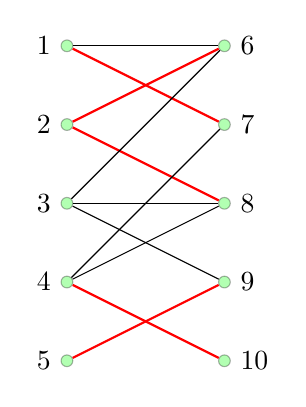
\begin{tikzpicture}
                \node[circle, draw=black, inner sep=1.5pt, fill=green, opacity=0.3, label={180:1}] (1) at (0, 0) {};
                \node[circle, draw=black, inner sep=1.5pt, fill=green, opacity=0.3, label={180:2}] (2) at (0, -1) {};
                \node[circle, draw=black, inner sep=1.5pt, fill=green, opacity=0.3, label={180:3}] (3) at (0, -2) {};
                \node[circle, draw=black, inner sep=1.5pt, fill=green, opacity=0.3, label={180:4}] (4) at (0, -3) {};
                \node[circle, draw=black, inner sep=1.5pt, fill=green, opacity=0.3, label={180:5}] (5) at (0, -4) {};
                \node[circle, draw=black, inner sep=1.5pt, fill=green, opacity=0.3, label={0:6}] (6) at (2, 0) {};
                \node[circle, draw=black, inner sep=1.5pt, fill=green, opacity=0.3, label={0:7}] (7) at (2, -1) {};
                \node[circle, draw=black, inner sep=1.5pt, fill=green, opacity=0.3, label={0:8}] (8) at (2, -2) {};
                \node[circle, draw=black, inner sep=1.5pt, fill=green, opacity=0.3, label={0:9}] (9) at (2, -3) {};
                \node[circle, draw=black, inner sep=1.5pt, fill=green, opacity=0.3, label={0:10}] (10) at (2, -4) {};
            
                \draw (1) -- (6);
                \draw[red, thick] (1) -- (7);
                \draw[red, thick] (2) -- (6);
                \draw[red, thick] (2) -- (8);
                \draw (3) -- (6);
                \draw (3) -- (8);
                \draw (3) -- (9);
                \draw (4) -- (7);
                \draw (4) -- (8);
                \draw[red, thick] (4) -- (10);
                \draw[red, thick] (5) -- (9);
            \end{tikzpicture}
            \caption{Not a matching- vertex 2 has 2 matching edges}
        \end{subfigure}
        \hfill
        \begin{subfigure}{0.45\textwidth}
            \centering
            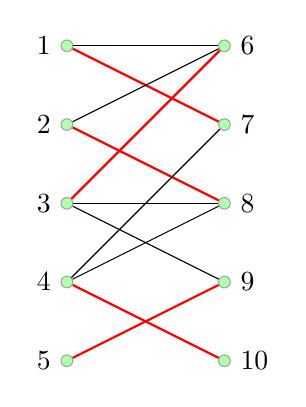
\begin{tikzpicture}
                \node[circle, draw=black, inner sep=1.5pt, fill=green, opacity=0.3, label={180:1}] (1) at (0, 0) {};
                \node[circle, draw=black, inner sep=1.5pt, fill=green, opacity=0.3, label={180:2}] (2) at (0, -1) {};
                \node[circle, draw=black, inner sep=1.5pt, fill=green, opacity=0.3, label={180:3}] (3) at (0, -2) {};
                \node[circle, draw=black, inner sep=1.5pt, fill=green, opacity=0.3, label={180:4}] (4) at (0, -3) {};
                \node[circle, draw=black, inner sep=1.5pt, fill=green, opacity=0.3, label={180:5}] (5) at (0, -4) {};
                \node[circle, draw=black, inner sep=1.5pt, fill=green, opacity=0.3, label={0:6}] (6) at (2, 0) {};
                \node[circle, draw=black, inner sep=1.5pt, fill=green, opacity=0.3, label={0:7}] (7) at (2, -1) {};
                \node[circle, draw=black, inner sep=1.5pt, fill=green, opacity=0.3, label={0:8}] (8) at (2, -2) {};
                \node[circle, draw=black, inner sep=1.5pt, fill=green, opacity=0.3, label={0:9}] (9) at (2, -3) {};
                \node[circle, draw=black, inner sep=1.5pt, fill=green, opacity=0.3, label={0:10}] (10) at (2, -4) {};
            
                \draw (1) -- (6);
                \draw[red, thick] (1) -- (7);
                \draw (2) -- (6);
                \draw[red, thick] (2) -- (8);
                \draw[red, thick] (3) -- (6);
                \draw (3) -- (8);
                \draw (3) -- (9);
                \draw (4) -- (7);
                \draw (4) -- (8);
                \draw[red, thick] (4) -- (10);
                \draw[red, thick] (5) -- (9);
            \end{tikzpicture}
            \caption{A matching}
        \end{subfigure}
    \end{figure}
    \noindent A \emph{maximum cardinality matching} is a matching that has the highest number of edges. A maximum matching is \emph{perfect} if it has cardinality $|V|/2$, i.e. every vertex is part of some edge in the matching. The example above shows a perfect matching. Not every bipartile graph has a perfect matching, such as the graph below:
    \begin{figure}[H]
        \centering
        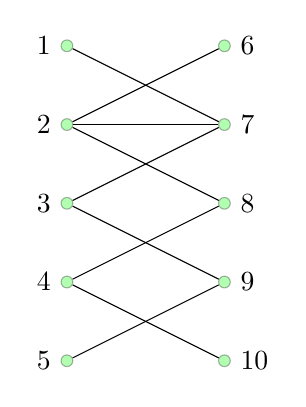
\begin{tikzpicture}
            \node[circle, draw=black, inner sep=1.5pt, fill=green, opacity=0.3, label={180:1}] (1) at (0, 0) {};
            \node[circle, draw=black, inner sep=1.5pt, fill=green, opacity=0.3, label={180:2}] (2) at (0, -1) {};
            \node[circle, draw=black, inner sep=1.5pt, fill=green, opacity=0.3, label={180:3}] (3) at (0, -2) {};
            \node[circle, draw=black, inner sep=1.5pt, fill=green, opacity=0.3, label={180:4}] (4) at (0, -3) {};
            \node[circle, draw=black, inner sep=1.5pt, fill=green, opacity=0.3, label={180:5}] (5) at (0, -4) {};
            \node[circle, draw=black, inner sep=1.5pt, fill=green, opacity=0.3, label={0:6}] (6) at (2, 0) {};
            \node[circle, draw=black, inner sep=1.5pt, fill=green, opacity=0.3, label={0:7}] (7) at (2, -1) {};
            \node[circle, draw=black, inner sep=1.5pt, fill=green, opacity=0.3, label={0:8}] (8) at (2, -2) {};
            \node[circle, draw=black, inner sep=1.5pt, fill=green, opacity=0.3, label={0:9}] (9) at (2, -3) {};
            \node[circle, draw=black, inner sep=1.5pt, fill=green, opacity=0.3, label={0:10}] (10) at (2, -4) {};
        
            \draw (1) -- (7);
            \draw (2) -- (6);
            \draw (2) -- (7);
            \draw (2) -- (8);
            \draw (3) -- (7);
            \draw (3) -- (9);
            \draw (4) -- (8);
            \draw (4) -- (10);
            \draw (5) -- (9);
        \end{tikzpicture}
    \end{figure}
    \noindent We will prove this by a contradiction. So, assume that this graph has a perfect matching. In that case, every vertex with just 1 edge will be part of the matching subset. This means that the red edges given below are part of the matching subset:
    \begin{figure}[H]
        \centering
        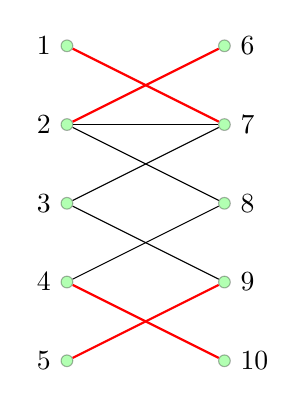
\begin{tikzpicture}
            \node[circle, draw=black, inner sep=1.5pt, fill=green, opacity=0.3, label={180:1}] (1) at (0, 0) {};
            \node[circle, draw=black, inner sep=1.5pt, fill=green, opacity=0.3, label={180:2}] (2) at (0, -1) {};
            \node[circle, draw=black, inner sep=1.5pt, fill=green, opacity=0.3, label={180:3}] (3) at (0, -2) {};
            \node[circle, draw=black, inner sep=1.5pt, fill=green, opacity=0.3, label={180:4}] (4) at (0, -3) {};
            \node[circle, draw=black, inner sep=1.5pt, fill=green, opacity=0.3, label={180:5}] (5) at (0, -4) {};
            \node[circle, draw=black, inner sep=1.5pt, fill=green, opacity=0.3, label={0:6}] (6) at (2, 0) {};
            \node[circle, draw=black, inner sep=1.5pt, fill=green, opacity=0.3, label={0:7}] (7) at (2, -1) {};
            \node[circle, draw=black, inner sep=1.5pt, fill=green, opacity=0.3, label={0:8}] (8) at (2, -2) {};
            \node[circle, draw=black, inner sep=1.5pt, fill=green, opacity=0.3, label={0:9}] (9) at (2, -3) {};
            \node[circle, draw=black, inner sep=1.5pt, fill=green, opacity=0.3, label={0:10}] (10) at (2, -4) {};
        
            \draw[red, thick] (1) -- (7);
            \draw[red, thick] (2) -- (6);
            \draw (2) -- (7);
            \draw (2) -- (8);
            \draw (3) -- (7);
            \draw (3) -- (9);
            \draw (4) -- (8);
            \draw[red, thick] (4) -- (10);
            \draw[red, thick] (5) -- (9);
        \end{tikzpicture}
    \end{figure}
    \noindent Now, since there is a perfect matching, we must be able to add precisely one further edge that will incorporate both the vertices 3 and 8. However, there is no edge between 3 and 8, and adding any other edge would only incorporate one of the vertices (and break the match property). So, this graph does not have a perfect matching. In fact, what we have above is the maximum cardinality matching for the graph.
    
    We will now construct an algorithm to compute the edges that form a maximum cardinality matching. If we did this using brute force, we would need to go through all the permutation of the edges and check whether it is a matching, and if so, whether it is also the maximum (up to that point during the algorithm). This will take $O(m!)$ time, where $m$ is the number of edges in the graph, and is essentially intractable. 

    We shall now look for a better algorithm, which has complexity $O(m^3)$. This uses the concept of finding an \emph{augmenting path} in the current matching to increase, if possible, the size of the matching by 1. The advantage we have in this case is that if we cannot find an augmenting path, then we have found the maximum cardinality matching. At the start, we have an empty matching, from which we increment the size of the matching by 1 until this is not possible, by finding an augmenting path.

    Before defining an augmenting path, we illustrate how this works. So, assume that we are at the following matching:
    \begin{figure}[H]
        \centering
        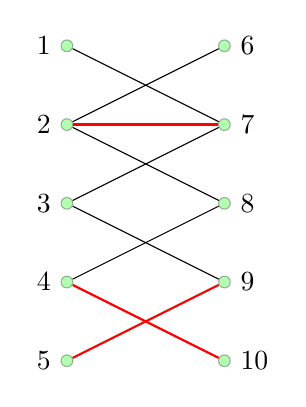
\begin{tikzpicture}
            \node[circle, draw=black, inner sep=1.5pt, fill=green, opacity=0.3, label={180:1}] (1) at (0, 0) {};
            \node[circle, draw=black, inner sep=1.5pt, fill=green, opacity=0.3, label={180:2}] (2) at (0, -1) {};
            \node[circle, draw=black, inner sep=1.5pt, fill=green, opacity=0.3, label={180:3}] (3) at (0, -2) {};
            \node[circle, draw=black, inner sep=1.5pt, fill=green, opacity=0.3, label={180:4}] (4) at (0, -3) {};
            \node[circle, draw=black, inner sep=1.5pt, fill=green, opacity=0.3, label={180:5}] (5) at (0, -4) {};
            \node[circle, draw=black, inner sep=1.5pt, fill=green, opacity=0.3, label={0:6}] (6) at (2, 0) {};
            \node[circle, draw=black, inner sep=1.5pt, fill=green, opacity=0.3, label={0:7}] (7) at (2, -1) {};
            \node[circle, draw=black, inner sep=1.5pt, fill=green, opacity=0.3, label={0:8}] (8) at (2, -2) {};
            \node[circle, draw=black, inner sep=1.5pt, fill=green, opacity=0.3, label={0:9}] (9) at (2, -3) {};
            \node[circle, draw=black, inner sep=1.5pt, fill=green, opacity=0.3, label={0:10}] (10) at (2, -4) {};
        
            \draw (1) -- (7);
            \draw (2) -- (6);
            \draw[red, thick] (2) -- (7);
            \draw (2) -- (8);
            \draw (3) -- (7);
            \draw (3) -- (9);
            \draw (4) -- (8);
            \draw[red, thick] (4) -- (10);
            \draw[red, thick] (5) -- (9);
        \end{tikzpicture}
    \end{figure}
    \noindent We can find an augmenting path here, which is shown below.
    \begin{figure}[H]
        \centering
        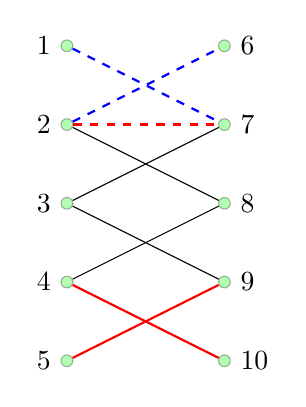
\begin{tikzpicture}
            \node[circle, draw=black, inner sep=1.5pt, fill=green, opacity=0.3, label={180:1}] (1) at (0, 0) {};
            \node[circle, draw=black, inner sep=1.5pt, fill=green, opacity=0.3, label={180:2}] (2) at (0, -1) {};
            \node[circle, draw=black, inner sep=1.5pt, fill=green, opacity=0.3, label={180:3}] (3) at (0, -2) {};
            \node[circle, draw=black, inner sep=1.5pt, fill=green, opacity=0.3, label={180:4}] (4) at (0, -3) {};
            \node[circle, draw=black, inner sep=1.5pt, fill=green, opacity=0.3, label={180:5}] (5) at (0, -4) {};
            \node[circle, draw=black, inner sep=1.5pt, fill=green, opacity=0.3, label={0:6}] (6) at (2, 0) {};
            \node[circle, draw=black, inner sep=1.5pt, fill=green, opacity=0.3, label={0:7}] (7) at (2, -1) {};
            \node[circle, draw=black, inner sep=1.5pt, fill=green, opacity=0.3, label={0:8}] (8) at (2, -2) {};
            \node[circle, draw=black, inner sep=1.5pt, fill=green, opacity=0.3, label={0:9}] (9) at (2, -3) {};
            \node[circle, draw=black, inner sep=1.5pt, fill=green, opacity=0.3, label={0:10}] (10) at (2, -4) {};
        
            \draw[blue, thick, dashed] (1) -- (7);
            \draw[blue, thick, dashed] (2) -- (6);
            \draw[red, dashed, thick] (2) -- (7);
            \draw (2) -- (8);
            \draw (3) -- (7);
            \draw (3) -- (9);
            \draw (4) -- (8);
            \draw[red, thick] (4) -- (10);
            \draw[red, thick] (5) -- (9);
        \end{tikzpicture}
    \end{figure}
    \noindent The augmenting path is the dashed path from the vertex 1 to 6 (or vice versa). An augmenting path alternates between edges in the match and not in the match, and helps us extend the cardinality of the matching. In this case, we remove the edge 2-7 from the matching (the dashed red edge), and replace it with 1-7 and 2-6 (the dashed blue edges). This gives us the following matching:
    \begin{figure}[H]
        \centering
        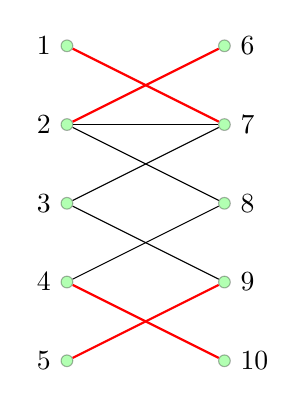
\begin{tikzpicture}
            \node[circle, draw=black, inner sep=1.5pt, fill=green, opacity=0.3, label={180:1}] (1) at (0, 0) {};
            \node[circle, draw=black, inner sep=1.5pt, fill=green, opacity=0.3, label={180:2}] (2) at (0, -1) {};
            \node[circle, draw=black, inner sep=1.5pt, fill=green, opacity=0.3, label={180:3}] (3) at (0, -2) {};
            \node[circle, draw=black, inner sep=1.5pt, fill=green, opacity=0.3, label={180:4}] (4) at (0, -3) {};
            \node[circle, draw=black, inner sep=1.5pt, fill=green, opacity=0.3, label={180:5}] (5) at (0, -4) {};
            \node[circle, draw=black, inner sep=1.5pt, fill=green, opacity=0.3, label={0:6}] (6) at (2, 0) {};
            \node[circle, draw=black, inner sep=1.5pt, fill=green, opacity=0.3, label={0:7}] (7) at (2, -1) {};
            \node[circle, draw=black, inner sep=1.5pt, fill=green, opacity=0.3, label={0:8}] (8) at (2, -2) {};
            \node[circle, draw=black, inner sep=1.5pt, fill=green, opacity=0.3, label={0:9}] (9) at (2, -3) {};
            \node[circle, draw=black, inner sep=1.5pt, fill=green, opacity=0.3, label={0:10}] (10) at (2, -4) {};
        
            \draw[red, thick] (1) -- (7);
            \draw[red, thick] (2) -- (6);
            \draw (2) -- (7);
            \draw (2) -- (8);
            \draw (3) -- (7);
            \draw (3) -- (9);
            \draw (4) -- (8);
            \draw[red, thick] (4) -- (10);
            \draw[red, thick] (5) -- (9);
        \end{tikzpicture}
    \end{figure}
    \noindent As we were able to find an augmenting path, we have been able to extend the matching subset by 1.

    We now build to the definition of augmenting path. In a matching $M$, we say that a vertex $v$ is \emph{matching} if it is part of some edge in the matching subset. If the edge goes from $v$ to $u$, then we say that $u$ and $v$ are \emph{mates}. If the vertex $v$ is not matched, then it is \emph{exposed}. An \emph{alternating path} alternates between edges in $M$ and edges not in $M$. An \emph{augmenting path} is an alternating path that starts and ends at exposed vertices.

    An augmenting path allows us to increase the length of the matching subset- an augmenting path has odd length (if it had even length, then it must end at an exposed vertex), so there is one more non-matching edge in the augmenting path than a matching edge. So, when we replace the matching edges with the non-matching edges, we still have a match (we are swapping the mates for the exposed vertices, and the unexposed vertices originally had no match). Moreover, if there is no augmenting path from any of the unexposed vertices, then we are at a maximum cardinality match.

    We will now consider the algorithm in general.
\begin{lstlisting}[language=pseudocode]
List<Edge> maximumMatching(Graph graph) {
    List<Edge> matching = [];
    Vertex augmentedPath = getAugmentedPath(graph.leftVertices);
    while (augmentedPath != null) {
        matching = augment(augmentedPath);
        augmentedPath = graph.getAugmentedPath();
    }
    return matching;
}
\end{lstlisting}
    The function \texttt{getAugmentedPath} tries to find an augmented path in the bipartile graph given its `left' vertices, and returns the final vertex in the path. The function \texttt{augment} takes an augmented path and selects the right edges to add to the matching.

    Next, we look at the method \texttt{getAugmentedPath} in detail. It is based on breadth-first search, starting from an unexposed vertex until we get to an unexposed vertex `on the same side'. As we saw in the algorithm above, we will only have a look at the left vertices. The following is the algorithm:
\begin{lstlisting}[language=pseudocode]
Vertex getAugmentedPath(List<Vertex> leftVertices) {
    Vertex startVertex = leftVertices.first((v) => v.isUnexposed);
    // no startVertex => every left vertex is exposed 
    if (startVertex == null) {
        return null;
    }

    // Do a DFS to find an unexposed vertex
    Queue<Vertex> queue = Queue(startVertex);
    while (queue.isNotEmpty) {
        Vertex vertex = queue.remove();
        List<Edge> edges = vertex.edges;

        for (int i=0; i<edges.length; i++) {
            Vertex range = edges[i].range;
            if (range.isVisited) {
                range.predecessorEdge = edges[i];
                if (range.isUnexposed) {
                    return range;
                } else {
                    queue.add(range.mate);
                }
            }
        }
    }

    // not possible to find a path between two unexposed vertices
    return null;
}
\end{lstlisting}
    We can then \texttt{augment} to find the matching path as follows:
\begin{lstlisting}[language=pseudocode]
List<Edge> augment(Vertex endVertex) {
    List<Edge> edges = [];
    Vertex vertex = endVertex;
    Edge edge = endVertex.predecessorEdge;

    while (edge != null) {
        Vertex temp = edge.range.mate;
        edge.range.mate = vertex;
        vertex.mate = edge.range;
        edges.add(edge);

        vertex = temp;
        edge = vertex.predecessorEdge;
    }

    return edges;
}
\end{lstlisting}
    Note that the variable \texttt{vertex} at line 12 cannot be null since it is on the left (and the path goes from a left vertex to another left vertex).

    We will now illustrate how the algorithm works with an example. So, assume that we have the following graph.
    \begin{figure}[H]
        \centering
        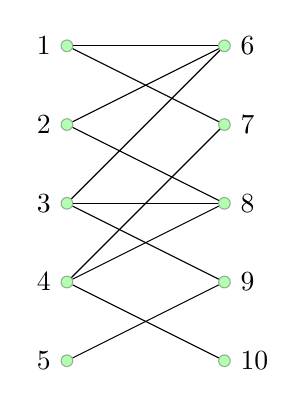
\begin{tikzpicture}
            \node[circle, draw=black, inner sep=1.5pt, fill=green, opacity=0.3, label={180:1}] (1) at (0, 0) {};
            \node[circle, draw=black, inner sep=1.5pt, fill=green, opacity=0.3, label={180:2}] (2) at (0, -1) {};
            \node[circle, draw=black, inner sep=1.5pt, fill=green, opacity=0.3, label={180:3}] (3) at (0, -2) {};
            \node[circle, draw=black, inner sep=1.5pt, fill=green, opacity=0.3, label={180:4}] (4) at (0, -3) {};
            \node[circle, draw=black, inner sep=1.5pt, fill=green, opacity=0.3, label={180:5}] (5) at (0, -4) {};
            \node[circle, draw=black, inner sep=1.5pt, fill=green, opacity=0.3, label={0:6}] (6) at (2, 0) {};
            \node[circle, draw=black, inner sep=1.5pt, fill=green, opacity=0.3, label={0:7}] (7) at (2, -1) {};
            \node[circle, draw=black, inner sep=1.5pt, fill=green, opacity=0.3, label={0:8}] (8) at (2, -2) {};
            \node[circle, draw=black, inner sep=1.5pt, fill=green, opacity=0.3, label={0:9}] (9) at (2, -3) {};
            \node[circle, draw=black, inner sep=1.5pt, fill=green, opacity=0.3, label={0:10}] (10) at (2, -4) {};
        
            \draw (1) -- (6);
            \draw (1) -- (7);
            \draw (2) -- (6);
            \draw (2) -- (8);
            \draw (3) -- (6);
            \draw (3) -- (8);
            \draw (3) -- (9);
            \draw (4) -- (7);
            \draw (4) -- (8);
            \draw (4) -- (10);
            \draw (5) -- (9);
        \end{tikzpicture}
    \end{figure}
    \noindent At the start, we have the empty matching. We will find an augmenting path in the graph.
    \begin{figure}[H]
        \centering
        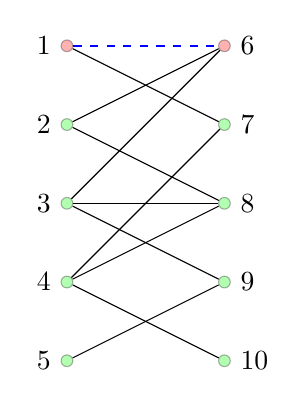
\begin{tikzpicture}
            \node[circle, draw=black, inner sep=1.5pt, fill=red, opacity=0.3, label={180:1}] (1) at (0, 0) {};
            \node[circle, draw=black, inner sep=1.5pt, fill=green, opacity=0.3, label={180:2}] (2) at (0, -1) {};
            \node[circle, draw=black, inner sep=1.5pt, fill=green, opacity=0.3, label={180:3}] (3) at (0, -2) {};
            \node[circle, draw=black, inner sep=1.5pt, fill=green, opacity=0.3, label={180:4}] (4) at (0, -3) {};
            \node[circle, draw=black, inner sep=1.5pt, fill=green, opacity=0.3, label={180:5}] (5) at (0, -4) {};
            \node[circle, draw=black, inner sep=1.5pt, fill=red, opacity=0.3, label={0:6}] (6) at (2, 0) {};
            \node[circle, draw=black, inner sep=1.5pt, fill=green, opacity=0.3, label={0:7}] (7) at (2, -1) {};
            \node[circle, draw=black, inner sep=1.5pt, fill=green, opacity=0.3, label={0:8}] (8) at (2, -2) {};
            \node[circle, draw=black, inner sep=1.5pt, fill=green, opacity=0.3, label={0:9}] (9) at (2, -3) {};
            \node[circle, draw=black, inner sep=1.5pt, fill=green, opacity=0.3, label={0:10}] (10) at (2, -4) {};
        
            \draw[blue, dashed, thick] (1) -- (6);
            \draw (1) -- (7);
            \draw (2) -- (6);
            \draw (2) -- (8);
            \draw (3) -- (6);
            \draw (3) -- (8);
            \draw (3) -- (9);
            \draw (4) -- (7);
            \draw (4) -- (8);
            \draw (4) -- (10);
            \draw (5) -- (9);
        \end{tikzpicture}
    \end{figure}
    \noindent We denote by red a visited vertex during this iteration. The first unexposed vertex we find is vertex 1, which has an edge to vertex 6. So, we add this edge to the matching. This gives us the following matching.
    \begin{figure}[H]
        \centering
        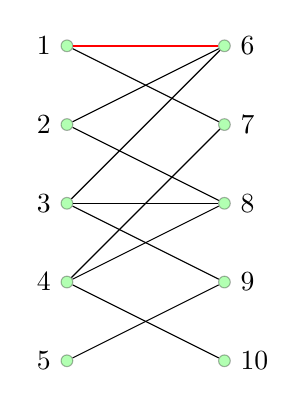
\begin{tikzpicture}
            \node[circle, draw=black, inner sep=1.5pt, fill=green, opacity=0.3, label={180:1}] (1) at (0, 0) {};
            \node[circle, draw=black, inner sep=1.5pt, fill=green, opacity=0.3, label={180:2}] (2) at (0, -1) {};
            \node[circle, draw=black, inner sep=1.5pt, fill=green, opacity=0.3, label={180:3}] (3) at (0, -2) {};
            \node[circle, draw=black, inner sep=1.5pt, fill=green, opacity=0.3, label={180:4}] (4) at (0, -3) {};
            \node[circle, draw=black, inner sep=1.5pt, fill=green, opacity=0.3, label={180:5}] (5) at (0, -4) {};
            \node[circle, draw=black, inner sep=1.5pt, fill=green, opacity=0.3, label={0:6}] (6) at (2, 0) {};
            \node[circle, draw=black, inner sep=1.5pt, fill=green, opacity=0.3, label={0:7}] (7) at (2, -1) {};
            \node[circle, draw=black, inner sep=1.5pt, fill=green, opacity=0.3, label={0:8}] (8) at (2, -2) {};
            \node[circle, draw=black, inner sep=1.5pt, fill=green, opacity=0.3, label={0:9}] (9) at (2, -3) {};
            \node[circle, draw=black, inner sep=1.5pt, fill=green, opacity=0.3, label={0:10}] (10) at (2, -4) {};
        
            \draw[red, thick] (1) -- (6);
            \draw (1) -- (7);
            \draw (2) -- (6);
            \draw (2) -- (8);
            \draw (3) -- (6);
            \draw (3) -- (8);
            \draw (3) -- (9);
            \draw (4) -- (7);
            \draw (4) -- (8);
            \draw (4) -- (10);
            \draw (5) -- (9);
        \end{tikzpicture}
    \end{figure}
    \noindent We will now search for another augmenting path.
    \begin{figure}[H]
        \centering
        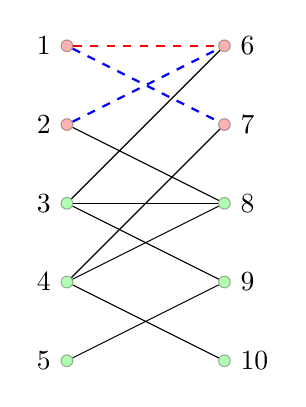
\begin{tikzpicture}
            \node[circle, draw=black, inner sep=1.5pt, fill=red, opacity=0.3, label={180:1}] (1) at (0, 0) {};
            \node[circle, draw=black, inner sep=1.5pt, fill=red, opacity=0.3, label={180:2}] (2) at (0, -1) {};
            \node[circle, draw=black, inner sep=1.5pt, fill=green, opacity=0.3, label={180:3}] (3) at (0, -2) {};
            \node[circle, draw=black, inner sep=1.5pt, fill=green, opacity=0.3, label={180:4}] (4) at (0, -3) {};
            \node[circle, draw=black, inner sep=1.5pt, fill=green, opacity=0.3, label={180:5}] (5) at (0, -4) {};
            \node[circle, draw=black, inner sep=1.5pt, fill=red, opacity=0.3, label={0:6}] (6) at (2, 0) {};
            \node[circle, draw=black, inner sep=1.5pt, fill=red, opacity=0.3, label={0:7}] (7) at (2, -1) {};
            \node[circle, draw=black, inner sep=1.5pt, fill=green, opacity=0.3, label={0:8}] (8) at (2, -2) {};
            \node[circle, draw=black, inner sep=1.5pt, fill=green, opacity=0.3, label={0:9}] (9) at (2, -3) {};
            \node[circle, draw=black, inner sep=1.5pt, fill=green, opacity=0.3, label={0:10}] (10) at (2, -4) {};
        
            \draw[red, dashed, thick] (1) -- (6);
            \draw[blue, dashed, thick] (1) -- (7);
            \draw[blue, dashed, thick] (2) -- (6);
            \draw (2) -- (8);
            \draw (3) -- (6);
            \draw (3) -- (8);
            \draw (3) -- (9);
            \draw (4) -- (7);
            \draw (4) -- (8);
            \draw (4) -- (10);
            \draw (5) -- (9);
        \end{tikzpicture}
    \end{figure}
    \noindent In this case, the augmenting path starts at vertex 2. We first find its edge to vertex 6. This is an exposed vertex, so we add its mate vertex 1 to the queue. From vertex 1, we cannot take the edge to vertex 6 since it has already been visited, so we take the edge to vertex 7. This vertex is exposed, so the augmenting path is complete. Using this, we get the following matching:
    \begin{figure}[H]
        \centering
        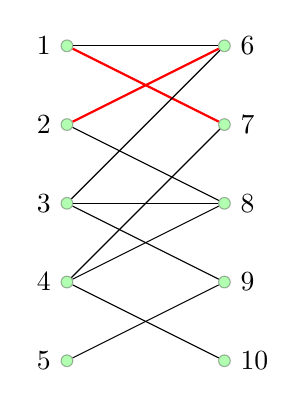
\begin{tikzpicture}
            \node[circle, draw=black, inner sep=1.5pt, fill=green, opacity=0.3, label={180:1}] (1) at (0, 0) {};
            \node[circle, draw=black, inner sep=1.5pt, fill=green, opacity=0.3, label={180:2}] (2) at (0, -1) {};
            \node[circle, draw=black, inner sep=1.5pt, fill=green, opacity=0.3, label={180:3}] (3) at (0, -2) {};
            \node[circle, draw=black, inner sep=1.5pt, fill=green, opacity=0.3, label={180:4}] (4) at (0, -3) {};
            \node[circle, draw=black, inner sep=1.5pt, fill=green, opacity=0.3, label={180:5}] (5) at (0, -4) {};
            \node[circle, draw=black, inner sep=1.5pt, fill=green, opacity=0.3, label={0:6}] (6) at (2, 0) {};
            \node[circle, draw=black, inner sep=1.5pt, fill=green, opacity=0.3, label={0:7}] (7) at (2, -1) {};
            \node[circle, draw=black, inner sep=1.5pt, fill=green, opacity=0.3, label={0:8}] (8) at (2, -2) {};
            \node[circle, draw=black, inner sep=1.5pt, fill=green, opacity=0.3, label={0:9}] (9) at (2, -3) {};
            \node[circle, draw=black, inner sep=1.5pt, fill=green, opacity=0.3, label={0:10}] (10) at (2, -4) {};
        
            \draw (1) -- (6);
            \draw[red, thick] (1) -- (7);
            \draw[red, thick] (2) -- (6);
            \draw (2) -- (8);
            \draw (3) -- (6);
            \draw (3) -- (8);
            \draw (3) -- (9);
            \draw (4) -- (7);
            \draw (4) -- (8);
            \draw (4) -- (10);
            \draw (5) -- (9);
        \end{tikzpicture}
    \end{figure}
    \noindent We can continue using the augmenting algorithm to get to the following matching:
    \begin{figure}[H]
        \centering
        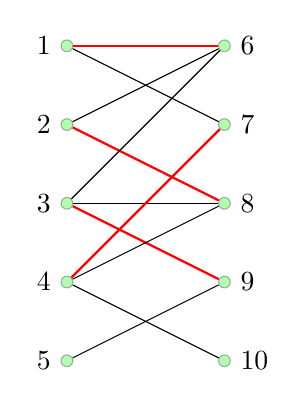
\begin{tikzpicture}
            \node[circle, draw=black, inner sep=1.5pt, fill=green, opacity=0.3, label={180:1}] (1) at (0, 0) {};
            \node[circle, draw=black, inner sep=1.5pt, fill=green, opacity=0.3, label={180:2}] (2) at (0, -1) {};
            \node[circle, draw=black, inner sep=1.5pt, fill=green, opacity=0.3, label={180:3}] (3) at (0, -2) {};
            \node[circle, draw=black, inner sep=1.5pt, fill=green, opacity=0.3, label={180:4}] (4) at (0, -3) {};
            \node[circle, draw=black, inner sep=1.5pt, fill=green, opacity=0.3, label={180:5}] (5) at (0, -4) {};
            \node[circle, draw=black, inner sep=1.5pt, fill=green, opacity=0.3, label={0:6}] (6) at (2, 0) {};
            \node[circle, draw=black, inner sep=1.5pt, fill=green, opacity=0.3, label={0:7}] (7) at (2, -1) {};
            \node[circle, draw=black, inner sep=1.5pt, fill=green, opacity=0.3, label={0:8}] (8) at (2, -2) {};
            \node[circle, draw=black, inner sep=1.5pt, fill=green, opacity=0.3, label={0:9}] (9) at (2, -3) {};
            \node[circle, draw=black, inner sep=1.5pt, fill=green, opacity=0.3, label={0:10}] (10) at (2, -4) {};
        
            \draw[red, thick] (1) -- (6);
            \draw (1) -- (7);
            \draw (2) -- (6);
            \draw[red, thick] (2) -- (8);
            \draw (3) -- (6);
            \draw (3) -- (8);
            \draw[red, thick] (3) -- (9);
            \draw[red, thick] (4) -- (7);
            \draw (4) -- (8);
            \draw (4) -- (10);
            \draw (5) -- (9);
        \end{tikzpicture}
    \end{figure}    
    \noindent Now, we will try finding another augmenting path.
    \begin{figure}[H]
        \centering
        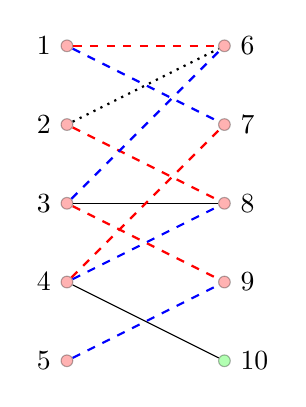
\begin{tikzpicture}
            \node[circle, draw=black, inner sep=1.5pt, fill=red, opacity=0.3, label={180:1}] (1) at (0, 0) {};
            \node[circle, draw=black, inner sep=1.5pt, fill=red, opacity=0.3, label={180:2}] (2) at (0, -1) {};
            \node[circle, draw=black, inner sep=1.5pt, fill=red, opacity=0.3, label={180:3}] (3) at (0, -2) {};
            \node[circle, draw=black, inner sep=1.5pt, fill=red, opacity=0.3, label={180:4}] (4) at (0, -3) {};
            \node[circle, draw=black, inner sep=1.5pt, fill=red, opacity=0.3, label={180:5}] (5) at (0, -4) {};
            \node[circle, draw=black, inner sep=1.5pt, fill=red, opacity=0.3, label={0:6}] (6) at (2, 0) {};
            \node[circle, draw=black, inner sep=1.5pt, fill=red, opacity=0.3, label={0:7}] (7) at (2, -1) {};
            \node[circle, draw=black, inner sep=1.5pt, fill=red, opacity=0.3, label={0:8}] (8) at (2, -2) {};
            \node[circle, draw=black, inner sep=1.5pt, fill=red, opacity=0.3, label={0:9}] (9) at (2, -3) {};
            \node[circle, draw=black, inner sep=1.5pt, fill=green, opacity=0.3, label={0:10}] (10) at (2, -4) {};
        
            \draw[red, dashed, thick] (1) -- (6);
            \draw[blue, dashed, thick] (1) -- (7);
            \draw[dotted, thick] (2) -- (6);
            \draw[red, dashed, thick] (2) -- (8);
            \draw[blue, thick, dashed] (3) -- (6);
            \draw (3) -- (8);
            \draw[red, dashed, thick] (3) -- (9);
            \draw[red, dashed, thick] (4) -- (7);
            \draw[blue, dashed, thick] (4) -- (8);
            \draw (4) -- (10);
            \draw[blue, thick, dashed] (5) -- (9);
        \end{tikzpicture}
    \end{figure}
    \noindent We start with the unexposed vertex 5, and take its edge to vertex 9. This is exposed, so we add its mate to the queue. This process continues as expected, until we add vertex 4 to the queue. We first take the edge it has to vertex 8, at which point we add vertex 3 to the queue. However, every edge that vertex 2 has goes to a visited vertex. So, we have to backtrack- we take the other edge from vertex 4.
    \begin{figure}[H]
        \centering
        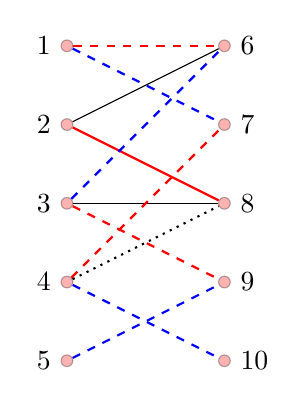
\begin{tikzpicture}
            \node[circle, draw=black, inner sep=1.5pt, fill=red, opacity=0.3, label={180:1}] (1) at (0, 0) {};
            \node[circle, draw=black, inner sep=1.5pt, fill=red, opacity=0.3, label={180:2}] (2) at (0, -1) {};
            \node[circle, draw=black, inner sep=1.5pt, fill=red, opacity=0.3, label={180:3}] (3) at (0, -2) {};
            \node[circle, draw=black, inner sep=1.5pt, fill=red, opacity=0.3, label={180:4}] (4) at (0, -3) {};
            \node[circle, draw=black, inner sep=1.5pt, fill=red, opacity=0.3, label={180:5}] (5) at (0, -4) {};
            \node[circle, draw=black, inner sep=1.5pt, fill=red, opacity=0.3, label={0:6}] (6) at (2, 0) {};
            \node[circle, draw=black, inner sep=1.5pt, fill=red, opacity=0.3, label={0:7}] (7) at (2, -1) {};
            \node[circle, draw=black, inner sep=1.5pt, fill=red, opacity=0.3, label={0:8}] (8) at (2, -2) {};
            \node[circle, draw=black, inner sep=1.5pt, fill=red, opacity=0.3, label={0:9}] (9) at (2, -3) {};
            \node[circle, draw=black, inner sep=1.5pt, fill=red, opacity=0.3, label={0:10}] (10) at (2, -4) {};
        
            \draw[red, dashed, thick] (1) -- (6);
            \draw[blue, dashed, thick] (1) -- (7);
            \draw (2) -- (6);
            \draw[red, thick] (2) -- (8);
            \draw[blue, thick, dashed] (3) -- (6);
            \draw (3) -- (8);
            \draw[red, dashed, thick] (3) -- (9);
            \draw[red, dashed, thick] (4) -- (7);
            \draw[thick, dotted] (4) -- (8);
            \draw[blue, dashed, thick] (4) -- (10);
            \draw[blue, thick, dashed] (5) -- (9);
        \end{tikzpicture}
    \end{figure}
    \noindent In this case, we take the edge from vertex 4 to vertex 10. This is an exposed vertex, so we have found the augmenting path. Moreover, there is no unexposed (left) vertex, so the algorithm terminates with the following matching:
    \begin{figure}[H]
        \centering
        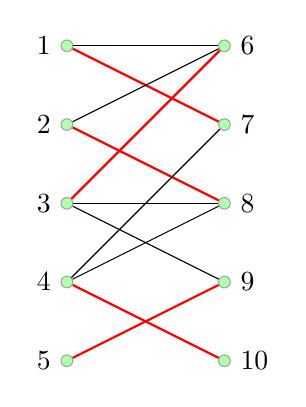
\begin{tikzpicture}
            \node[circle, draw=black, inner sep=1.5pt, fill=green, opacity=0.3, label={180:1}] (1) at (0, 0) {};
            \node[circle, draw=black, inner sep=1.5pt, fill=green, opacity=0.3, label={180:2}] (2) at (0, -1) {};
            \node[circle, draw=black, inner sep=1.5pt, fill=green, opacity=0.3, label={180:3}] (3) at (0, -2) {};
            \node[circle, draw=black, inner sep=1.5pt, fill=green, opacity=0.3, label={180:4}] (4) at (0, -3) {};
            \node[circle, draw=black, inner sep=1.5pt, fill=green, opacity=0.3, label={180:5}] (5) at (0, -4) {};
            \node[circle, draw=black, inner sep=1.5pt, fill=green, opacity=0.3, label={0:6}] (6) at (2, 0) {};
            \node[circle, draw=black, inner sep=1.5pt, fill=green, opacity=0.3, label={0:7}] (7) at (2, -1) {};
            \node[circle, draw=black, inner sep=1.5pt, fill=green, opacity=0.3, label={0:8}] (8) at (2, -2) {};
            \node[circle, draw=black, inner sep=1.5pt, fill=green, opacity=0.3, label={0:9}] (9) at (2, -3) {};
            \node[circle, draw=black, inner sep=1.5pt, fill=green, opacity=0.3, label={0:10}] (10) at (2, -4) {};
        
            \draw (1) -- (6);
            \draw[red, thick] (1) -- (7);
            \draw (2) -- (6);
            \draw[red, thick] (2) -- (8);
            \draw[red, thick] (3) -- (6);
            \draw (3) -- (8);
            \draw (3) -- (9);
            \draw (4) -- (7);
            \draw (4) -- (8);
            \draw[red, thick] (4) -- (10);
            \draw[red, thick] (5) -- (9);
        \end{tikzpicture}
    \end{figure}

    We will now consider the complexity of the algorithm. Assume that $p$ and $q$ are the number of vertices in the two partitions of the graph, and let $|V| = n$ and $|E| = m$. We assume that $p < q$, with $p$ the number of left vertices without loss of generality. The function \texttt{getAugmentedPath} is a version of depth-first search where every second vertex is a left vertex, so it has $O(p + m)$ complexity. The augmenting process has $O(m)$ complexity since we encounter an edge at most once during the iteration. The main loop can run at most $p$ times- during each iteration, we must expose a left vertex. So, the entire algorithm takes $O(p(p+m))$ time. We have $p \leq n$, so this is $O(n(n+m))$. If we further assume that $m = O(n^2)$, we find that the algorithm is $O(n^3)$. The fastest algorithm that is known has complexity $O(\sqrt{n}(n+m))$, and this complexity can also be achieved for non-bipartile graphs.
    \newpage

    \section{Network Flow}
    In this section, we will look at a network (which is a special kind of directed graph), which has a (maximum) capacity along with a flow (a weighted graph) that obeys some rules. We will consider how to compute the maximum flow for a given network.

    A \emph{network} is a directed graph $G = (V, E)$ such that there is a \emph{source} vertex (which has no incoming edge) and a \emph{sink} (which has no outgoing edge), and every edge $(u, v) \in E$ has a non-negative \emph{capacity}, denoted by $c(u, v) \in \mathbb{R}$. For two vertices $u$ and $v$ without any edge between them, we can define their capacity $c(u, v) = 0$. A \emph{flow} in a network $G$ is a function $f \colon E \to \mathbb{R}$ such that it obeys the following:
    \begin{itemize}
        \item capacity constraint: for every edge $(u, v) \in E$, $0 \leq f(u, v) \leq c(u, v)$, i.e. the flow doesn't exceed the capacity; and
        \item flow conservation constraint: for every vertex $v$ that is not the source or the sink, the total incoming flow equals the total outgoing flow.
    \end{itemize}
    The \emph{value} of a flow $f$, denoted by $f$, is the total outgoing flow from the source $s$ (or the total incoming flow to the sink $t$).

    The following example gives a network, with the values denoting the capacity of each edge.
    \begin{figure}[H]
        \centering
        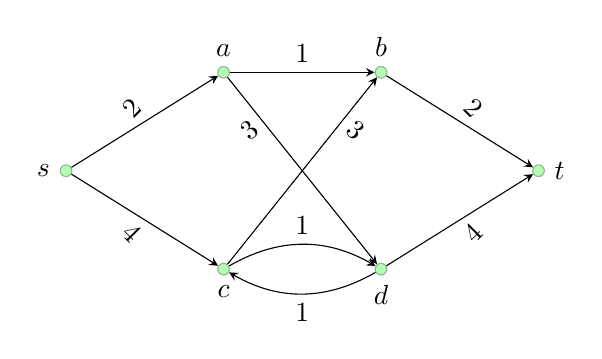
\begin{tikzpicture}
            \node[circle, draw, inner sep=1.5pt, fill=green, opacity=0.3, label={-180:$s$}] (s) at (0, 0) {};
            \node[circle, draw, inner sep=1.5pt, fill=green, opacity=0.3, label={90:$a$}] (a) at (2, 1.25) {};
            \node[circle, draw, inner sep=1.5pt, fill=green, opacity=0.3, label={90:$b$}] (b) at (4, 1.25) {};
            \node[circle, draw, inner sep=1.5pt, fill=green, opacity=0.3, label={-90:$c$}] (c) at (2, -1.25) {};
            \node[circle, draw, inner sep=1.5pt, fill=green, opacity=0.3, label={-90:$d$}] (d) at (4, -1.25) {};
            \node[circle, draw, inner sep=1.5pt, fill=green, opacity=0.3, label={0:$t$}] (t) at (6, 0) {};

            \draw[-stealth] (s) -- node[above, rotate=45] {2} (a);
            \draw[-stealth] (s) -- node[below, rotate=-45] {4} (c);
            \draw[-stealth] (a) -- node[above] {1} (b);
            \draw[-stealth] (b) -- node[above, rotate=-45] {2} (t);
            \draw[-stealth] (d) -- node[below, rotate=45] {4} (t);
            \draw[-stealth] (a) -- node[below left, rotate=40, pos=0.15] {3} (d);
            \draw[-stealth] (c) -- node[below right, rotate=-40, pos=0.85] {3} (b);
            \draw[-stealth] (c) edge[bend left] node[above] {1} (d);
            \draw[-stealth] (d) edge[bend left] node[below] {1} (c);
        \end{tikzpicture}
    \end{figure}
    \noindent A possible flow through the network is the following:
    \begin{figure}[H]
        \centering
        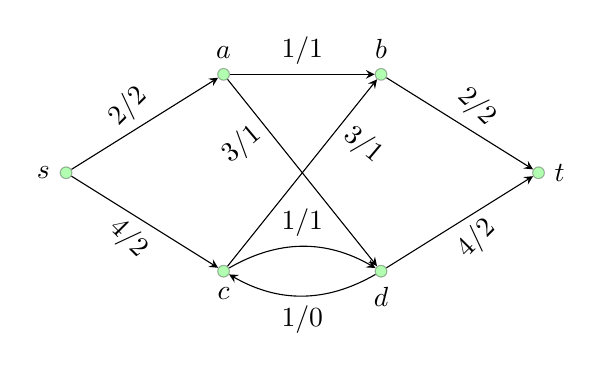
\begin{tikzpicture}
            \node[circle, draw, inner sep=1.5pt, fill=green, opacity=0.3, label={-180:$s$}] (s) at (0, 0) {};
            \node[circle, draw, inner sep=1.5pt, fill=green, opacity=0.3, label={90:$a$}] (a) at (2, 1.25) {};
            \node[circle, draw, inner sep=1.5pt, fill=green, opacity=0.3, label={90:$b$}] (b) at (4, 1.25) {};
            \node[circle, draw, inner sep=1.5pt, fill=green, opacity=0.3, label={-90:$c$}] (c) at (2, -1.25) {};
            \node[circle, draw, inner sep=1.5pt, fill=green, opacity=0.3, label={-90:$d$}] (d) at (4, -1.25) {};
            \node[circle, draw, inner sep=1.5pt, fill=green, opacity=0.3, label={0:$t$}] (t) at (6, 0) {};

            \draw[-stealth] (s) -- node[above, rotate=45] {2/2} (a);
            \draw[-stealth] (s) -- node[below, rotate=-45] {4/2} (c);
            \draw[-stealth] (a) -- node[above] {1/1} (b);
            \draw[-stealth] (b) -- node[above, rotate=-45] {2/2} (t);
            \draw[-stealth] (d) -- node[below, rotate=45] {4/2} (t);
            \draw[-stealth] (a) -- node[below left, rotate=40, pos=0.15] {3/1} (d);
            \draw[-stealth] (c) -- node[below right, rotate=-40, pos=0.85] {3/1} (b);
            \draw[-stealth] (c) edge[bend left] node[above] {1/1} (d);
            \draw[-stealth] (d) edge[bend left] node[below] {1/0} (c);
        \end{tikzpicture}
    \end{figure}
    \noindent We denote an edge by $a/b$, where $a$ is the capacity and $b$ is the flow. We can see that the flow is always non-negative and smaller than the capacity. Moreover, for $a$, $b$, $c$ and $d$, the total incoming flow equals the total outgoing flow, e.g. $s-a$ is the only incoming edge to $a$, with flow $2$, and the two outgoing edges $a - b$ and $a - d$ have total flow $2$. The value of the flow above is 4. We can actually find another flow of higher value. Consider the flow given below:
    \begin{figure}[H]
        \centering
        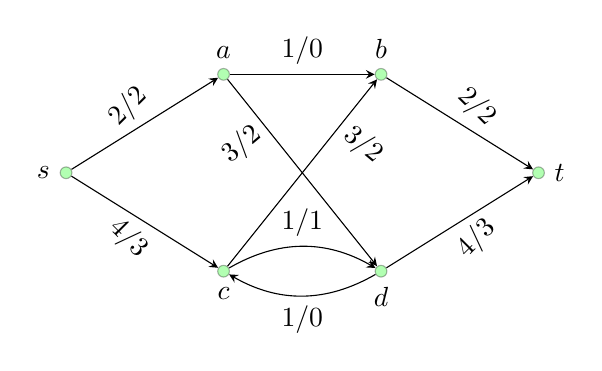
\begin{tikzpicture}
            \node[circle, draw, inner sep=1.5pt, fill=green, opacity=0.3, label={-180:$s$}] (s) at (0, 0) {};
            \node[circle, draw, inner sep=1.5pt, fill=green, opacity=0.3, label={90:$a$}] (a) at (2, 1.25) {};
            \node[circle, draw, inner sep=1.5pt, fill=green, opacity=0.3, label={90:$b$}] (b) at (4, 1.25) {};
            \node[circle, draw, inner sep=1.5pt, fill=green, opacity=0.3, label={-90:$c$}] (c) at (2, -1.25) {};
            \node[circle, draw, inner sep=1.5pt, fill=green, opacity=0.3, label={-90:$d$}] (d) at (4, -1.25) {};
            \node[circle, draw, inner sep=1.5pt, fill=green, opacity=0.3, label={0:$t$}] (t) at (6, 0) {};

            \draw[-stealth] (s) -- node[above, rotate=45] {2/2} (a);
            \draw[-stealth] (s) -- node[below, rotate=-45] {4/3} (c);
            \draw[-stealth] (a) -- node[above] {1/0} (b);
            \draw[-stealth] (b) -- node[above, rotate=-45] {2/2} (t);
            \draw[-stealth] (d) -- node[below, rotate=45] {4/3} (t);
            \draw[-stealth] (a) -- node[below left, rotate=40, pos=0.15] {3/2} (d);
            \draw[-stealth] (c) -- node[below right, rotate=-40, pos=0.85] {3/2} (b);
            \draw[-stealth] (c) edge[bend left] node[above] {1/1} (d);
            \draw[-stealth] (d) edge[bend left] node[below] {1/0} (c);
        \end{tikzpicture}
    \end{figure}
    \noindent We can verify by inspection that we have a flow above. Moreover, it has value 5.
    
    We claim that there is no flow of higher value. Assume, for a contradiction, that there is a flow of value 6. We try to construct such a flow:
    \begin{figure}[H]
        \centering
        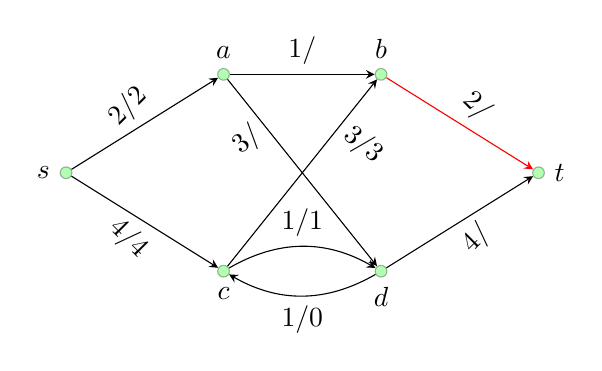
\begin{tikzpicture}
            \node[circle, draw, inner sep=1.5pt, fill=green, opacity=0.3, label={-180:$s$}] (s) at (0, 0) {};
            \node[circle, draw, inner sep=1.5pt, fill=green, opacity=0.3, label={90:$a$}] (a) at (2, 1.25) {};
            \node[circle, draw, inner sep=1.5pt, fill=green, opacity=0.3, label={90:$b$}] (b) at (4, 1.25) {};
            \node[circle, draw, inner sep=1.5pt, fill=green, opacity=0.3, label={-90:$c$}] (c) at (2, -1.25) {};
            \node[circle, draw, inner sep=1.5pt, fill=green, opacity=0.3, label={-90:$d$}] (d) at (4, -1.25) {};
            \node[circle, draw, inner sep=1.5pt, fill=green, opacity=0.3, label={0:$t$}] (t) at (6, 0) {};

            \draw[-stealth] (s) -- node[above, rotate=45] {2/2} (a);
            \draw[-stealth] (s) -- node[below, rotate=-45] {4/4} (c);
            \draw[-stealth] (a) -- node[above] {1/} (b);
            \draw[-stealth, red] (b) -- node[black, above, rotate=-45] {2/} (t);
            \draw[-stealth] (d) -- node[below, rotate=45] {4/} (t);
            \draw[-stealth] (a) -- node[below left, rotate=40, pos=0.15] {3/} (d);
            \draw[-stealth] (c) -- node[below right, rotate=-40, pos=0.85] {3/3} (b);
            \draw[-stealth] (c) edge[bend left] node[above] {1/1} (d);
            \draw[-stealth] (d) edge[bend left] node[below] {1/0} (c);
        \end{tikzpicture}
    \end{figure}
    \noindent Since the sources have total outgoing capacity 6, the outgoing edges from $s$ must be \emph{saturated} (capacity equals flow). This means that $c$ has incoming flow of at least 4. Since the outgoing edges have total capacity 4, the edge $c - d$ has flow 0. Also, the outgoing edges from $c$ must be saturated. In particular, $b$ has incoming flow of at least 3. However, $b$ only has one outgoing edge (given in red), with capacity 2. This is a contradiction- we cannot have a flow of value 6. So, the flow we had above of value 5 is the maximum flow.

    We will now look at an algorithm to find a maximum flow for a network. To do so, we will need to use \emph{augmenting paths}, like in the maximum cardinality matching algorithm. An augmenting path is a path from the source $s$ to the sink $t$ that has edges in $G$, but not necessarily in the direction that it exists in $G$. In particular, an edge $(u, v)$ in the path satisfies one of the following:
    \begin{itemize}
        \item $(u, v)$ is an edge in $G$, and the flow is not equal to the capacity (this is a \emph{forwards-edge})- the difference is called the \emph{slack}, which is greater than 0; or
        \item $(v, u)$ is an edge in $G$, and the flow is non-zero (this is a \emph{backwards-edge}).
    \end{itemize}
    Using an augmented path, we can increase the value of the flow- we increase the flow in the forwards-edges (while ensuring it doesn't cross the capacity) and decrease the flow in backwards-edges (while ensuring it doesn't go below 0). The following is an augmenting path for the network we had above:    
    \begin{figure}[H]
        \centering
        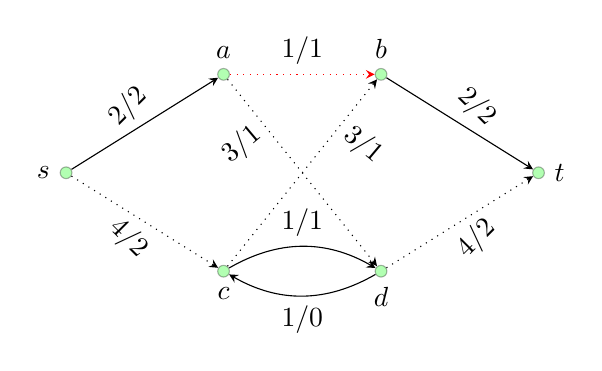
\begin{tikzpicture}
            \node[circle, draw, inner sep=1.5pt, fill=green, opacity=0.3, label={-180:$s$}] (s) at (0, 0) {};
            \node[circle, draw, inner sep=1.5pt, fill=green, opacity=0.3, label={90:$a$}] (a) at (2, 1.25) {};
            \node[circle, draw, inner sep=1.5pt, fill=green, opacity=0.3, label={90:$b$}] (b) at (4, 1.25) {};
            \node[circle, draw, inner sep=1.5pt, fill=green, opacity=0.3, label={-90:$c$}] (c) at (2, -1.25) {};
            \node[circle, draw, inner sep=1.5pt, fill=green, opacity=0.3, label={-90:$d$}] (d) at (4, -1.25) {};
            \node[circle, draw, inner sep=1.5pt, fill=green, opacity=0.3, label={0:$t$}] (t) at (6, 0) {};

            \draw[-stealth] (s) -- node[above, rotate=45] {2/2} (a);
            \draw[-stealth, dotted] (s) -- node[below, rotate=-45] {4/2} (c);
            \draw[-stealth, red, dotted] (a) -- node[above, black] {1/1} (b);
            \draw[-stealth] (b) -- node[above, rotate=-45] {2/2} (t);
            \draw[-stealth, dotted] (d) -- node[below, rotate=45] {4/2} (t);
            \draw[-stealth, dotted] (a) -- node[below left, rotate=40, pos=0.15] {3/1} (d);
            \draw[-stealth, dotted] (c) -- node[below right, rotate=-40, pos=0.85] {3/1} (b);
            \draw[-stealth] (c) edge[bend left] node[above] {1/1} (d);
            \draw[-stealth] (d) edge[bend left] node[below] {1/0} (c);
        \end{tikzpicture}
    \end{figure}
    \noindent The network has flow 4. The augmenting path has 5 edges: $(s, c)$, $(c, b)$, $(b, a)$, $(a, d)$ and $(d, t)$. Only the edge $(b, a)$ is backwards (and given in red). The edge $(s, c)$ has slack 2; the edge $(c, d)$ has slack 2; the flow in the edge $(b, a)$ can be decreased by 1, and so on. We compute the minimum value $m$ corresponding to an edge and change the flow accordingly- we increment the flow by $m$ to a forwards-edge and decrement by $m$ to a backwards-edge. This gives us the following network flow:
    \begin{figure}[H]
        \centering
        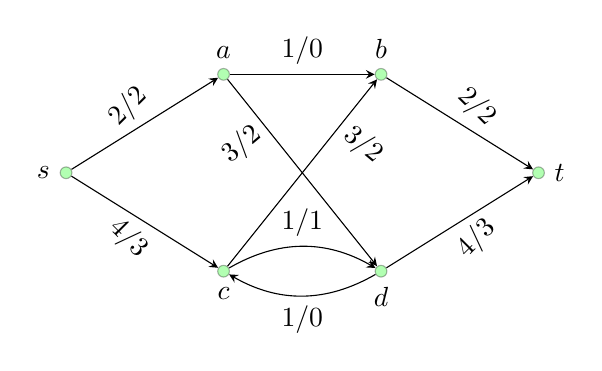
\begin{tikzpicture}
            \node[circle, draw, inner sep=1.5pt, fill=green, opacity=0.3, label={-180:$s$}] (s) at (0, 0) {};
            \node[circle, draw, inner sep=1.5pt, fill=green, opacity=0.3, label={90:$a$}] (a) at (2, 1.25) {};
            \node[circle, draw, inner sep=1.5pt, fill=green, opacity=0.3, label={90:$b$}] (b) at (4, 1.25) {};
            \node[circle, draw, inner sep=1.5pt, fill=green, opacity=0.3, label={-90:$c$}] (c) at (2, -1.25) {};
            \node[circle, draw, inner sep=1.5pt, fill=green, opacity=0.3, label={-90:$d$}] (d) at (4, -1.25) {};
            \node[circle, draw, inner sep=1.5pt, fill=green, opacity=0.3, label={0:$t$}] (t) at (6, 0) {};

            \draw[-stealth] (s) -- node[above, rotate=45] {2/2} (a);
            \draw[-stealth] (s) -- node[below, rotate=-45] {4/3} (c);
            \draw[-stealth] (a) -- node[above] {1/0} (b);
            \draw[-stealth] (b) -- node[above, rotate=-45] {2/2} (t);
            \draw[-stealth] (d) -- node[below, rotate=45] {4/3} (t);
            \draw[-stealth] (a) -- node[below left, rotate=40, pos=0.15] {3/2} (d);
            \draw[-stealth] (c) -- node[below right, rotate=-40, pos=0.85] {3/2} (b);
            \draw[-stealth] (c) edge[bend left] node[above] {1/1} (d);
            \draw[-stealth] (d) edge[bend left] node[below] {1/0} (c);
        \end{tikzpicture}
    \end{figure}
    \noindent This flow has value 5. Every edge leaving the source has to be a forwards-edge (if there was a backwards-edge, then there would be an incoming edge to the source, which is not possible). Hence, the value of the flow must always increase when we augment the flow using the augmenting path.

    Like in the case of the maximum cardinality matching algorithm, a flow is maximum if and only if it has no augmenting path. We saw above that if the flow has an augmenting path, then it is not maximum- we can change the flow by the minimum of the slack/flow so that the value of the flow increases.

    In particular, let $m$ be the minimum of the slacks for forwards edges and flow for backwards edges. We have a new function $f' \colon E \to \mathbb{R}$, based on the previous flow function $f \colon E \to \mathbb{R}$. We will now show $f'$ is actually a flow, i.e. it obeys the capacity and the flow-conservation constraint. First, we consider the capacity constraint:
    \begin{itemize}
        \item the flow we generate will keep the edges not in the augmenting path the same, so they obey the flow capacity constraint;
        \item a forwards-edge has its flow increased at most by its slack, so it is at most the capacity;
        \item a backwards-edge has its flow decreased at most by the previous flow, so it is at least 0. 
    \end{itemize}
    So, the capacity constraint is always satisfied. For a vertex (not the source or the sink) that has no edges in the augmenting path, it still satisfies the flow-conservation constraint. Instead, if a vertex $v$ is part of some edge in the augmenting path, then it must be part of two edges. We have two choices for each edge- a forwards-edge and a backwards-edge. We consider each case separately:
    \begin{itemize}
        \item if we have two forwards-edges, then the edges in $E$ are $(u, v)$ and $(v, w)$, as given below:
        \begin{figure}[H]
            \centering
            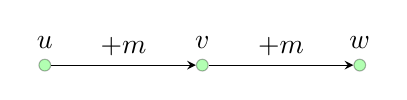
\begin{tikzpicture}
                \node[circle, draw, inner sep=1.5pt, fill=green, opacity=0.3, label={90:$u$}] (u) at (0, 0) {};
                \node[circle, draw, inner sep=1.5pt, fill=green, opacity=0.3, label={90:$v$}] (v) at (2, 0.0) {};
                \node[circle, draw, inner sep=1.5pt, fill=green, opacity=0.3, label={90:$w$}] (w) at (4, 0.0) {};

                \draw[-stealth] (u) -- node[above] {$+m$} (v);
                \draw[-stealth] (v) -- node[above] {$+m$} (w);
            \end{tikzpicture}
        \end{figure}
        \noindent So, the incoming flow and the outgoing flow for $v$ increases by $m$, so given that the flow was conserved for $v$ originally, it is still conserved.

        \item if we have a forwards-edge and a backwards-edge, then the edges in $E$ are $(u, v)$ and $(w, v)$, as given below:
        \begin{figure}[H]
            \centering
            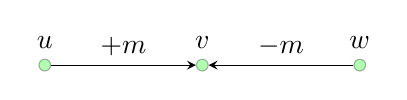
\begin{tikzpicture}
                \node[circle, draw, inner sep=1.5pt, fill=green, opacity=0.3, label={90:$u$}] (u) at (0, 0) {};
                \node[circle, draw, inner sep=1.5pt, fill=green, opacity=0.3, label={90:$v$}] (v) at (2, 0.0) {};
                \node[circle, draw, inner sep=1.5pt, fill=green, opacity=0.3, label={90:$w$}] (w) at (4, 0.0) {};

                \draw[-stealth] (u) -- node[above] {$+m$} (v);
                \draw[-stealth] (w) -- node[above] {$-m$} (v);
            \end{tikzpicture}
        \end{figure}
        \noindent By the edge $(u, v)$, the flow increases by $m$; by the edge $(w, v)$, the flow decreases by $m$. Hence, the incoming flow for $v$ doesn't change, i.e. it is still conserved.
    \end{itemize}
    We can use the same idea for the other two cases. So, the flow is conserved in each case. We have also seen above that the value of the new flow $f'$ is $m > 0$ more than the value of the flow $f$. Hence, $f$ is not a maximum flow.

    To prove the other direction, we introduce the concept of a cut. A \emph{cut} in a network is a set of edges in $E$ such that removing those edges means we no longer have a path from the source to the sink. For example, consider the following network:
    \begin{figure}[H]
        \centering
        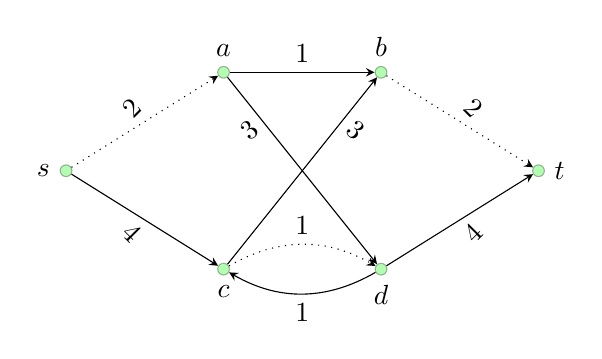
\begin{tikzpicture}
            \node[circle, draw, inner sep=1.5pt, fill=green, opacity=0.3, label={-180:$s$}] (s) at (0, 0) {};
            \node[circle, draw, inner sep=1.5pt, fill=green, opacity=0.3, label={90:$a$}] (a) at (2, 1.25) {};
            \node[circle, draw, inner sep=1.5pt, fill=green, opacity=0.3, label={90:$b$}] (b) at (4, 1.25) {};
            \node[circle, draw, inner sep=1.5pt, fill=green, opacity=0.3, label={-90:$c$}] (c) at (2, -1.25) {};
            \node[circle, draw, inner sep=1.5pt, fill=green, opacity=0.3, label={-90:$d$}] (d) at (4, -1.25) {};
            \node[circle, draw, inner sep=1.5pt, fill=green, opacity=0.3, label={0:$t$}] (t) at (6, 0) {};

            \draw[-stealth, dotted] (s) -- node[above, rotate=45] {2} (a);
            \draw[-stealth] (s) -- node[below, rotate=-45] {4} (c);
            \draw[-stealth] (a) -- node[above] {1} (b);
            \draw[-stealth, dotted] (b) -- node[above, rotate=-45] {2} (t);
            \draw[-stealth] (d) -- node[below, rotate=45] {4} (t);
            \draw[-stealth] (a) -- node[below left, rotate=40, pos=0.15] {3} (d);
            \draw[-stealth] (c) -- node[below right, rotate=-40, pos=0.85] {3} (b);
            \draw[-stealth, dotted] (c) edge[bend left] node[above] {1} (d);
            \draw[-stealth] (d) edge[bend left] node[below] {1} (c);
        \end{tikzpicture}
    \end{figure}
    \noindent The values given for each edge represents its capacity. In the graph above, if we remove the dotted edges, then we can no longer travel from the source $s$ to the sink $t$- we get stuck at $b$. We can also define cuts in a different way- consider a partition of the vertex set into the sets $A$ and $B$, where the source $s \in A$ and the sink $t \in B$. We can define a cut as follows:
    \[C = A \times B \cap E = \{(u, v) \in E \mid u \in A, v \in B\}.\]
    In the graph above, the cut $C$ has $A = \{s, b, c\}$ and $B = \{t, a, d\}$. We define the capacity of a cut $C$ by the sum of the capacity of the edges in it. So, in the example above, we have $\operatorname{cap}(C) = 5$.

    % We can show that the two definitions of the cut are equivalent. We will show one direction- if we remove the edges at the cut $C$, then there is no path from the source to the sink. Assume, for a contradiction, that there is a path from the source to the sink. Denote the path as follows: $(s, e_1), (e_1, e_2), \dots, (e_r, t)$. We know that $s \in A$. Since $(s, e_1)$ remains in the graph, the edge cannot be in $C$. Hence, $e_1 \in A$. Using this argument inductively, we find that $e_r \in A$. This would imply that $t \in A$. However, we must have $t \in B$. This is a contradiction. So, there is no path from the source to the sink.

    We now return to the proof of the Augmenting Path Theorem. In particular, we want to show that if a network has no augmenting path, then it is a maximum flow. We do this by constructing a cut with capacity equal to the capacity of the network flow. Then, we can make use of the Max-Cut Min-Flow theorem\sidefootnote{The Max-Cut Min-Flow theorem states that the value of a maximum flow is equal to the capacity of some minimum cut.}  to show that the network flow has maximum capacity. Intuitively, this follows since the cut ensures that no addition flow can pass from the source to the sink, hence the current flow is maximal.

    Let $G = (V, E)$ be the network, with source $s$ and sink $t$. We define a \emph{partial augmenting path} to be a path that is like an augmenting path, but does not end at the sink. Let $A \subseteq V$ be the set of partial augmenting paths and $B = V \setminus A$. We know that there is no augmenting path in $G$, so we know that $t \not\in A$, i.e. $t \in B$. Furthermore, the trivial path gives us $s \in A$. So, we define the cut as follows:
    \[C = \{(u, v) \in E \mid u \in A, v \in B\}.\]
    For an edge $(u, v) \in C$ with $(u, v) \in E$, we claim that the flow $f(u, v)$ equals capacity- otherwise, we can get a valid edge from $u$ to $v$, which gives us a partial augmenting path, i.e. $v \in A$. Similarly, for $(u, v) \in C$ with $(v, u) \in E$, we claim that the flow $f(v, u) = 0$- we get the same contradiction otherwise. This implies that the capacity of the cut equals the capacity of the flow, so the flow is maximum. 

    Above, we saw that the following is a maximum network flow:
    \begin{figure}[H]
        \centering
        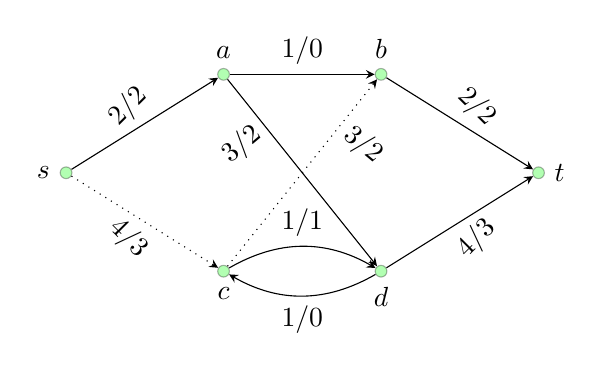
\begin{tikzpicture}
            \node[circle, draw, inner sep=1.5pt, fill=green, opacity=0.3, label={-180:$s$}] (s) at (0, 0) {};
            \node[circle, draw, inner sep=1.5pt, fill=green, opacity=0.3, label={90:$a$}] (a) at (2, 1.25) {};
            \node[circle, draw, inner sep=1.5pt, fill=green, opacity=0.3, label={90:$b$}] (b) at (4, 1.25) {};
            \node[circle, draw, inner sep=1.5pt, fill=green, opacity=0.3, label={-90:$c$}] (c) at (2, -1.25) {};
            \node[circle, draw, inner sep=1.5pt, fill=green, opacity=0.3, label={-90:$d$}] (d) at (4, -1.25) {};
            \node[circle, draw, inner sep=1.5pt, fill=green, opacity=0.3, label={0:$t$}] (t) at (6, 0) {};

            \draw[-stealth] (s) -- node[above, rotate=45] {2/2} (a);
            \draw[-stealth, dotted] (s) -- node[below, rotate=-45] {4/3} (c);
            \draw[-stealth] (a) -- node[above] {1/0} (b);
            \draw[-stealth] (b) -- node[above, rotate=-45] {2/2} (t);
            \draw[-stealth] (d) -- node[below, rotate=45] {4/3} (t);
            \draw[-stealth] (a) -- node[below left, rotate=40, pos=0.15] {3/2} (d);
            \draw[-stealth, dotted] (c) -- node[below right, rotate=-40, pos=0.85] {3/2} (b);
            \draw[-stealth] (c) edge[bend left] node[above] {1/1} (d);
            \draw[-stealth] (d) edge[bend left] node[below] {1/0} (c);
        \end{tikzpicture}
    \end{figure}
    \noindent The dotted edges give us all the vertices we can reach from $s$. Using this, we can define the partitions $A = \{s, c, b\}$ and $B = \{a, d, t\}$. Then, the cut generated by $A$ and $B$ is the following:
    \begin{figure}[H]
        \centering
        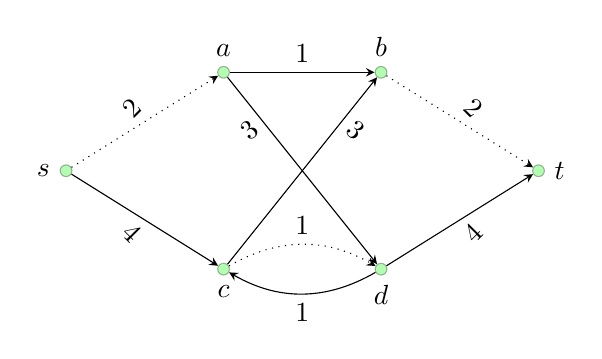
\begin{tikzpicture}
            \node[circle, draw, inner sep=1.5pt, fill=green, opacity=0.3, label={-180:$s$}] (s) at (0, 0) {};
            \node[circle, draw, inner sep=1.5pt, fill=green, opacity=0.3, label={90:$a$}] (a) at (2, 1.25) {};
            \node[circle, draw, inner sep=1.5pt, fill=green, opacity=0.3, label={90:$b$}] (b) at (4, 1.25) {};
            \node[circle, draw, inner sep=1.5pt, fill=green, opacity=0.3, label={-90:$c$}] (c) at (2, -1.25) {};
            \node[circle, draw, inner sep=1.5pt, fill=green, opacity=0.3, label={-90:$d$}] (d) at (4, -1.25) {};
            \node[circle, draw, inner sep=1.5pt, fill=green, opacity=0.3, label={0:$t$}] (t) at (6, 0) {};

            \draw[-stealth, dotted] (s) -- node[above, rotate=45] {2} (a);
            \draw[-stealth] (s) -- node[below, rotate=-45] {4} (c);
            \draw[-stealth] (a) -- node[above] {1} (b);
            \draw[-stealth, dotted] (b) -- node[above, rotate=-45] {2} (t);
            \draw[-stealth] (d) -- node[below, rotate=45] {4} (t);
            \draw[-stealth] (a) -- node[below left, rotate=40, pos=0.15] {3} (d);
            \draw[-stealth] (c) -- node[below right, rotate=-40, pos=0.85] {3} (b);
            \draw[-stealth, dotted] (c) edge[bend left] node[above] {1} (d);
            \draw[-stealth] (d) edge[bend left] node[below] {1} (c);
        \end{tikzpicture}
    \end{figure}
    \noindent The dotted lines show the edges part of the cut. The capacity of this cut is 5, which equals the capacity of the network flow.

    We will now look at the algorithm to find the maximum flow. This is given by the Ford-Fulkerson algorithm. Superficially, the algorithm is the same as for the maximum cardinality matching- we start up with the empty flow and use augmenting paths to increase the flow capacity, until there is no augmenting path.

    We search for augmenting paths using the residual graph. It is a directed weighted graph (not necessarily a network) that we can traverse to find an augmenting path. For instance, we have an example of a flow and its residual graph below.        
    \begin{figure}[H]
        \centering
        \begin{subfigure}{0.48\textwidth}
            \begin{scalebox}{0.8}{
                \centering
                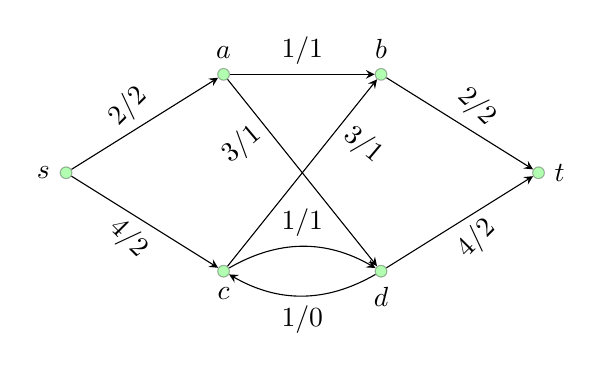
\begin{tikzpicture}
                    \node[circle, draw, inner sep=1.5pt, fill=green, opacity=0.3, label={-180:$s$}] (s) at (0, 0) {};
                    \node[circle, draw, inner sep=1.5pt, fill=green, opacity=0.3, label={90:$a$}] (a) at (2, 1.25) {};
                    \node[circle, draw, inner sep=1.5pt, fill=green, opacity=0.3, label={90:$b$}] (b) at (4, 1.25) {};
                    \node[circle, draw, inner sep=1.5pt, fill=green, opacity=0.3, label={-90:$c$}] (c) at (2, -1.25) {};
                    \node[circle, draw, inner sep=1.5pt, fill=green, opacity=0.3, label={-90:$d$}] (d) at (4, -1.25) {};
                    \node[circle, draw, inner sep=1.5pt, fill=green, opacity=0.3, label={0:$t$}] (t) at (6, 0) {};

                    \draw[-stealth] (s) -- node[above, rotate=45] {2/2} (a);
                    \draw[-stealth] (s) -- node[below, rotate=-45] {4/2} (c);
                    \draw[-stealth] (a) -- node[above] {1/1} (b);
                    \draw[-stealth] (b) -- node[above, rotate=-45] {2/2} (t);
                    \draw[-stealth] (d) -- node[below, rotate=45] {4/2} (t);
                    \draw[-stealth] (a) -- node[below left, rotate=40, pos=0.15] {3/1} (d);
                    \draw[-stealth] (c) -- node[below right, rotate=-40, pos=0.85] {3/1} (b);
                    \draw[-stealth] (c) edge[bend left] node[above] {1/1} (d);
                    \draw[-stealth] (d) edge[bend left] node[below] {1/0} (c);
                \end{tikzpicture}
                }
            \end{scalebox}
        \end{subfigure}
        \hfill
        \begin{subfigure}{0.48\textwidth}
            \begin{scalebox}{0.8}{
                \centering
                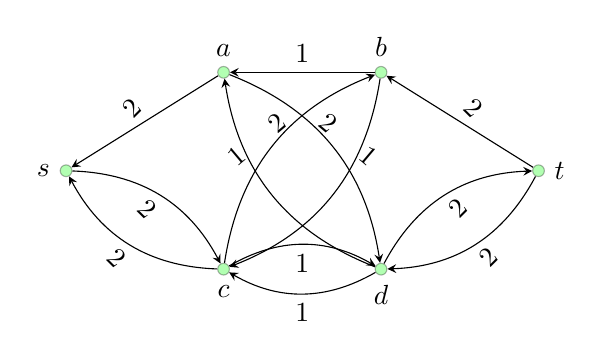
\begin{tikzpicture}
                    \node[circle, draw, inner sep=1.5pt, fill=green, opacity=0.3, label={-180:$s$}] (s) at (0, 0) {};
                    \node[circle, draw, inner sep=1.5pt, fill=green, opacity=0.3, label={90:$a$}] (a) at (2, 1.25) {};
                    \node[circle, draw, inner sep=1.5pt, fill=green, opacity=0.3, label={90:$b$}] (b) at (4, 1.25) {};
                    \node[circle, draw, inner sep=1.5pt, fill=green, opacity=0.3, label={-90:$c$}] (c) at (2, -1.25) {};
                    \node[circle, draw, inner sep=1.5pt, fill=green, opacity=0.3, label={-90:$d$}] (d) at (4, -1.25) {};
                    \node[circle, draw, inner sep=1.5pt, fill=green, opacity=0.3, label={0:$t$}] (t) at (6, 0) {};

                    \draw[-stealth] (a) -- node[above, rotate=45] {2} (s);
                    \draw[-stealth] (s) edge[bend left] node[below, rotate=-45] {2} (c);
                    \draw[-stealth] (c) edge[bend left] node[below, rotate=-45] {2} (s);
                    \draw[-stealth] (b) -- node[above] {1} (a);
                    \draw[-stealth] (t) -- node[above, rotate=-45] {2} (b);
                    \draw[-stealth] (d) edge[bend left] node[below, rotate=45] {2} (t);
                    \draw[-stealth] (t) edge[bend left] node[below, rotate=45] {2} (d);
                    \draw[-stealth] (a) edge[bend left] node[below left, rotate=40, pos=0.2] {2} (d);
                    \draw[-stealth] (d) edge[bend left] node[below left, rotate=40, pos=0.8] {1} (a);
                    \draw[-stealth] (c) edge[bend left] node[below right, rotate=-40, pos=0.8] {2} (b);
                    \draw[-stealth] (b) edge[bend left] node[below right, rotate=-40, pos=0.2] {1} (c);
                    \draw[-stealth] (d) edge[bend left] node[below] {1} (c);
                    \draw[-stealth] (c) edge[bend left] node[below] {1} (d);
                \end{tikzpicture}
                }
            \end{scalebox}
        \end{subfigure}
    \end{figure}
    \noindent The vertex set in the network and the residue graph is identical. For an edge $(u, v) \in E$, if its flow $f(u, v)$ is smaller than the capacity $c(u, v)$, then there is an edge $(u, v)$ in the residue with weight equal to the slack. Also, if the flow $f(u, v)$ is greater than zero, then there is an edge $(v, u)$ in the residue with weight equal to the flow. In the case above, there are 2 ways we can get the edge $(d, c)$ in the residual graph- a forwards-edge and a backwards-edge. This can be represented in many ways- the flow can be equal to one of them, the sum of them, or be represented by multiple edges. We shall always choose one of them.

    To find an augmenting path, we traverse the residue path, starting from the source and ending up at the sink. We can use an algorithm such as depth-first search or breadth-first search to find the path. The edges that are part of the path will lead to an augmenting path. We illustrate this with the network/residue above.
    \begin{figure}[H]
        \centering
        \begin{subfigure}{0.45\textwidth}
            \begin{scalebox}{0.8}{
                \centering
                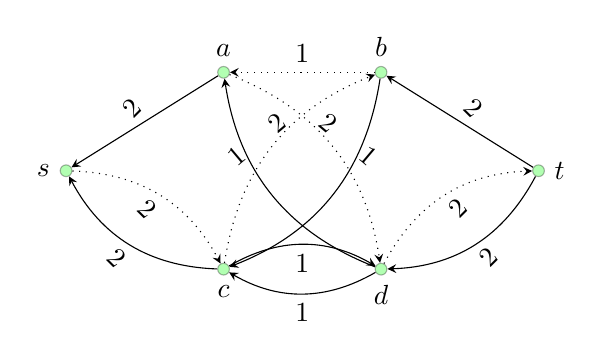
\begin{tikzpicture}
                    \node[circle, draw, inner sep=1.5pt, fill=green, opacity=0.3, label={-180:$s$}] (s) at (0, 0) {};
                    \node[circle, draw, inner sep=1.5pt, fill=green, opacity=0.3, label={90:$a$}] (a) at (2, 1.25) {};
                    \node[circle, draw, inner sep=1.5pt, fill=green, opacity=0.3, label={90:$b$}] (b) at (4, 1.25) {};
                    \node[circle, draw, inner sep=1.5pt, fill=green, opacity=0.3, label={-90:$c$}] (c) at (2, -1.25) {};
                    \node[circle, draw, inner sep=1.5pt, fill=green, opacity=0.3, label={-90:$d$}] (d) at (4, -1.25) {};
                    \node[circle, draw, inner sep=1.5pt, fill=green, opacity=0.3, label={0:$t$}] (t) at (6, 0) {};

                    \draw[-stealth] (a) -- node[above, rotate=45] {2} (s);
                    \draw[-stealth, dotted] (s) edge[bend left] node[below, rotate=-45] {2} (c);
                    \draw[-stealth] (c) edge[bend left] node[below, rotate=-45] {2} (s);
                    \draw[-stealth, dotted] (b) -- node[above] {1} (a);
                    \draw[-stealth] (t) -- node[above, rotate=-45] {2} (b);
                    \draw[-stealth, dotted] (d) edge[bend left] node[below, rotate=45] {2} (t);
                    \draw[-stealth] (t) edge[bend left] node[below, rotate=45] {2} (d);
                    \draw[-stealth, dotted] (a) edge[bend left] node[below left, rotate=40, pos=0.2] {2} (d);
                    \draw[-stealth] (d) edge[bend left] node[below left, rotate=40, pos=0.8] {1} (a);
                    \draw[-stealth, dotted] (c) edge[bend left] node[below right, rotate=-40, pos=0.8] {2} (b);
                    \draw[-stealth] (b) edge[bend left] node[below right, rotate=-40, pos=0.2] {1} (c);
                    \draw[-stealth] (d) edge[bend left] node[below] {1} (c);
                    \draw[-stealth] (c) edge[bend left] node[below] {1} (d);
                \end{tikzpicture}
                }
            \end{scalebox}
        \end{subfigure}
        \hfill
        \begin{subfigure}{0.45\textwidth}
            \centering
            \begin{scalebox}{0.8}{
                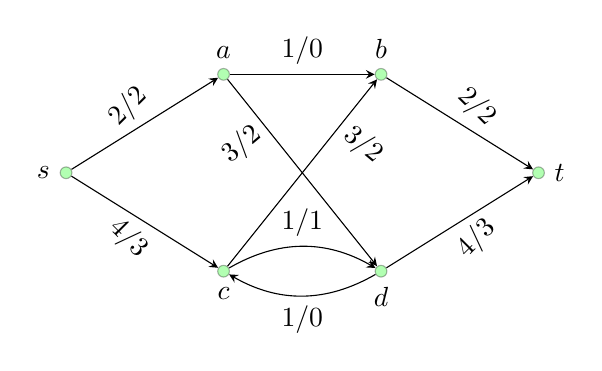
\begin{tikzpicture}
                    \node[circle, draw, inner sep=1.5pt, fill=green, opacity=0.3, label={-180:$s$}] (s) at (0, 0) {};
                    \node[circle, draw, inner sep=1.5pt, fill=green, opacity=0.3, label={90:$a$}] (a) at (2, 1.25) {};
                    \node[circle, draw, inner sep=1.5pt, fill=green, opacity=0.3, label={90:$b$}] (b) at (4, 1.25) {};
                    \node[circle, draw, inner sep=1.5pt, fill=green, opacity=0.3, label={-90:$c$}] (c) at (2, -1.25) {};
                    \node[circle, draw, inner sep=1.5pt, fill=green, opacity=0.3, label={-90:$d$}] (d) at (4, -1.25) {};
                    \node[circle, draw, inner sep=1.5pt, fill=green, opacity=0.3, label={0:$t$}] (t) at (6, 0) {};
        
                    \draw[-stealth] (s) -- node[above, rotate=45] {2/2} (a);
                    \draw[-stealth] (s) -- node[below, rotate=-45] {4/3} (c);
                    \draw[-stealth] (a) -- node[above] {1/0} (b);
                    \draw[-stealth] (b) -- node[above, rotate=-45] {2/2} (t);
                    \draw[-stealth] (d) -- node[below, rotate=45] {4/3} (t);
                    \draw[-stealth] (a) -- node[below left, rotate=40, pos=0.15] {3/2} (d);
                    \draw[-stealth] (c) -- node[below right, rotate=-40, pos=0.85] {3/2} (b);
                    \draw[-stealth] (c) edge[bend left] node[above] {1/1} (d);
                    \draw[-stealth] (d) edge[bend left] node[below] {1/0} (c);
                \end{tikzpicture}
                }
            \end{scalebox}
        \end{subfigure}
    \end{figure}
    \noindent The path in the residual graph is given on the left- it is: $(s, c)$, $(c, b)$, $(b, a)$, $(a, d)$ and $(d, t)$. This is an augmented path in the network. Using this augmented path, we can improve the flow. In this case, we increase the capacity by 1- this is given on the right.

    Below is the Ford-Fulkerson algorithm:
\begin{lstlisting}[language=pseudocode]
void fordFulkerson(Network network) {
    Graph graph = network.residue;
    List<Edge> edges = graph.augmentingPath;
    while (edges.isNotEmpty) {
        int m = edges.minVal;
        network.augment(edges, m);
        edges = graph.augmentingPath;
    }
}
\end{lstlisting}
    We assume that the network is initialised with flow equal to 0. The \texttt{augment} method changes the flow of an edge by $m$- a forwards-edge has its flow increased, while a backwards-edge has its flow decreased. We can find out whether an edge is a forwards-edge or a backwards-edge by checking whether it can be increased/decreased by $m$; we can also keep track of this using a boolean field.

    We will now consider the complexity of the algorithm. The initialisation is $O(|E|)$- we set the flow 0 to all the edges. The main loop iterates at most $O(\texttt{maxFlow})$ times (if the flow only ever increases by 1). To build the residual graph, it takes $O(|V| + |E|)$ time- we have the same number of vertices and (at most) double the edges. We can find an augmenting path in $O(|V| + |E|)$ time, e.g. using BFS or DFS. The augmentation changes the flow of the edges- it takes $O(|E|)$ time. If we assume that every vertex is on a directed path from $s$ to $t$, we find that $|V| = O(|E|)$. Hence, the algorithm has complexity $O(|E| \cdot \texttt{maxFlow})$. This is a pseudo-linear algorithm, which can be quite inefficient.

    The bound of \texttt{maxFlow} can be improved in some cases by choosing the right augmenting path. For example, consider the following network, with the given capacities:
    \begin{figure}[H]
        \centering
        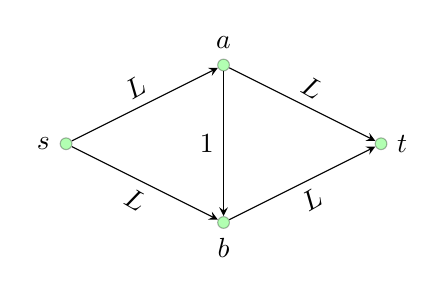
\begin{tikzpicture}
            \node[circle, draw, inner sep=1.5pt, fill=green, opacity=0.3, label={180:$s$}] (s) at (0, 0) {};
            \node[circle, draw, inner sep=1.5pt, fill=green, opacity=0.3, label={90:$a$}] (a) at (2, 1) {};
            \node[circle, draw, inner sep=1.5pt, fill=green, opacity=0.3, label={-90:$b$}] (b) at (2, -1) {};
            \node[circle, draw, inner sep=1.5pt, fill=green, opacity=0.3, label={0:$t$}] (t) at (4, 0) {};
            
            \draw[-stealth] (s) --  node[above, rotate=30] {$L$} (a);
            \draw[-stealth] (s) --  node[below, rotate=-30] {$L$} (b);
            \draw[-stealth] (a) -- node[above, rotate=-30] {$L$} (t);
            \draw[-stealth] (b) -- node[below, rotate=30] {$L$} (t);
            \draw[-stealth] (a) -- node[left] {1} (b);
        \end{tikzpicture}
    \end{figure}
    \noindent If we choose the path $(s, a), (a, b), (b, t)$, then we can only increase the capacity by 1. We can then choose the path $(s, b), (b, a), (a, t)$, the same thing happens. The algorithm might loop around these two choices, and only find the maximum flow after $2L$ iterations. However, we can find the maximum flow in just 2 iterations- take the edges $(s, a), (a, t)$ and $(s, b), (b, t)$. 
    
    We can get this improvement by always choosing the shortest augmenting path. This can be achieved using breadth-first search. If we use this version of the Ford-Fulkerson algorithm, then we are using the \emph{Edomons-Karp heuristic}. Using this version, we only search for an augmenting path $O(|V||E|)$ times, so the Ford-Fulkerson algorithm has complexity $O(|V||E|^2) = O(|E|^3)$. The fastest algorithm known has complexity $O(|V||E|)$.

    % \begin{figure}[H]
    %     \centering
    %     \begin{tikzpicture}
    %         \node[circle, draw, inner sep=1.5pt, fill=green, opacity=0.3, label={-180:$s$}] (s) at (0, 0) {};
    %         \node[circle, draw, inner sep=1.5pt, fill=green, opacity=0.3, label={90:$a$}] (a) at (2, 1.25) {};
    %         \node[circle, draw, inner sep=1.5pt, fill=green, opacity=0.3, label={90:$b$}] (b) at (4, 1.25) {};
    %         \node[circle, draw, inner sep=1.5pt, fill=green, opacity=0.3, label={-90:$c$}] (c) at (2, -1.25) {};
    %         \node[circle, draw, inner sep=1.5pt, fill=green, opacity=0.3, label={-90:$d$}] (d) at (4, -1.25) {};
    %         \node[circle, draw, inner sep=1.5pt, fill=green, opacity=0.3, label={0:$t$}] (t) at (6, 0) {};

    %         \draw[-stealth] (a) -- node[above, rotate=45] {2} (s);
    %         \draw[-stealth, dotted] (s) edge[bend left] node[below, rotate=-45] {1} (c);
    %         \draw[-stealth] (c) edge[bend left] node[below, rotate=-45] {3} (s);
    %         \draw[-stealth] (a) -- node[above] {1} (b);
    %         \draw[-stealth] (t) -- node[above, rotate=-45] {2} (b);
    %         \draw[-stealth] (d) edge[bend left] node[below, rotate=45] {1} (t);
    %         \draw[-stealth] (t) edge[bend left] node[below, rotate=45] {3} (d);
    %         \draw[-stealth] (a) edge[bend left] node[below left, rotate=40, pos=0.2] {1} (d);
    %         \draw[-stealth] (d) edge[bend left] node[below left, rotate=40, pos=0.8] {2} (a);
    %         \draw[-stealth, dotted] (c) edge[bend left] node[below right, rotate=-40, pos=0.8] {1} (b);
    %         \draw[-stealth] (b) edge[bend left] node[below right, rotate=-40, pos=0.2] {2} (c);
    %         \draw[-stealth] (d) edge[bend left] node[below] {1} (c);
    %         \draw[-stealth] (c) edge[bend left] node[below] {1} (d);
    %     \end{tikzpicture}
    % \end{figure}
    % TODO: 3600 onwards
    
    We will now illustrate how the algorithm works with an example. Assume we have the following network, with the given capacities:
    \begin{figure}[H]
        \centering
        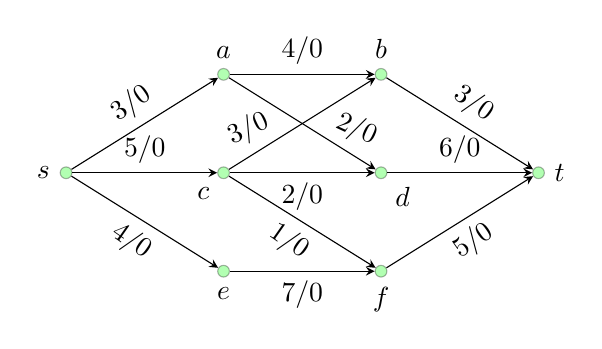
\begin{tikzpicture}
            \node[circle, draw, inner sep=1.5pt, fill=green, opacity=0.3, label={-180:$s$}] (s) at (0, 0) {};
            \node[circle, draw, inner sep=1.5pt, fill=green, opacity=0.3, label={90:$a$}] (a) at (2, 1.25) {};
            \node[circle, draw, inner sep=1.5pt, fill=green, opacity=0.3, label={90:$b$}] (b) at (4, 1.25) {};
            \node[circle, draw, inner sep=1.5pt, fill=green, opacity=0.3, label={-135:$c$}] (c) at (2, 0) {};
            \node[circle, draw, inner sep=1.5pt, fill=green, opacity=0.3, label={-45:$d$}] (d) at (4, 0) {};
            \node[circle, draw, inner sep=1.5pt, fill=green, opacity=0.3, label={-90:$e$}] (e) at (2, -1.25) {};
            \node[circle, draw, inner sep=1.5pt, fill=green, opacity=0.3, label={-90:$f$}] (f) at (4, -1.25) {};
            \node[circle, draw, inner sep=1.5pt, fill=green, opacity=0.3, label={0:$t$}] (t) at (6, 0) {};

            \draw[-stealth] (s) -- node[above, rotate=35] {$3/0$} (a);
            \draw[-stealth] (s) -- node[above] {$5/0$} (c);
            \draw[-stealth] (s) -- node[below, rotate=-35] {$4/0$} (e);
            \draw[-stealth] (a) -- node[above] {$4/0$} (b);
            \draw[-stealth] (e) -- node[below] {$7/0$} (f);
            \draw[-stealth] (b) -- node[above, rotate=-35] {$3/0$} (t);
            \draw[-stealth] (d) -- node[above] {$6/0$} (t);
            \draw[-stealth] (f) -- node[below, rotate=35] {$5/0$} (t);
            \draw[-stealth] (c) -- node[below] {$2/0$} (d);
            \draw[-stealth] (a) -- node[above, rotate=-25, pos=0.8] {$2/0$} (d);
            \draw[-stealth] (c) -- node[above, rotate=25, pos=0.2] {$3/0$} (b);
            \draw[-stealth] (c) -- node[below, rotate=-35] {$1/0$} (f);
        \end{tikzpicture}
    \end{figure}
    \noindent We initialise the flow with value 0, and construct the residual graph.
    \begin{figure}[H]
        \centering
        \begin{subfigure}{0.48\textwidth}
            \centering
            \scalebox{0.8}{
                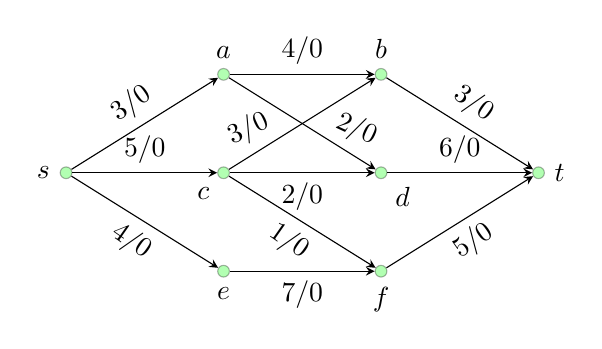
\begin{tikzpicture}
                    \node[circle, draw, inner sep=1.5pt, fill=green, opacity=0.3, label={-180:$s$}] (s) at (0, 0) {};
                    \node[circle, draw, inner sep=1.5pt, fill=green, opacity=0.3, label={90:$a$}] (a) at (2, 1.25) {};
                    \node[circle, draw, inner sep=1.5pt, fill=green, opacity=0.3, label={90:$b$}] (b) at (4, 1.25) {};
                    \node[circle, draw, inner sep=1.5pt, fill=green, opacity=0.3, label={-135:$c$}] (c) at (2, 0) {};
                    \node[circle, draw, inner sep=1.5pt, fill=green, opacity=0.3, label={-45:$d$}] (d) at (4, 0) {};
                    \node[circle, draw, inner sep=1.5pt, fill=green, opacity=0.3, label={-90:$e$}] (e) at (2, -1.25) {};
                    \node[circle, draw, inner sep=1.5pt, fill=green, opacity=0.3, label={-90:$f$}] (f) at (4, -1.25) {};
                    \node[circle, draw, inner sep=1.5pt, fill=green, opacity=0.3, label={0:$t$}] (t) at (6, 0) {};

                    \draw[-stealth] (s) -- node[above, rotate=35] {$3/0$} (a);
                    \draw[-stealth] (s) -- node[above] {$5/0$} (c);
                    \draw[-stealth] (s) -- node[below, rotate=-35] {$4/0$} (e);
                    \draw[-stealth] (a) -- node[above] {$4/0$} (b);
                    \draw[-stealth] (e) -- node[below] {$7/0$} (f);
                    \draw[-stealth] (b) -- node[above, rotate=-35] {$3/0$} (t);
                    \draw[-stealth] (d) -- node[above] {$6/0$} (t);
                    \draw[-stealth] (f) -- node[below, rotate=35] {$5/0$} (t);
                    \draw[-stealth] (c) -- node[below] {$2/0$} (d);
                    \draw[-stealth] (a) -- node[above, rotate=-25, pos=0.8] {$2/0$} (d);
                    \draw[-stealth] (c) -- node[above, rotate=25, pos=0.2] {$3/0$} (b);
                    \draw[-stealth] (c) -- node[below, rotate=-35] {$1/0$} (f);
                \end{tikzpicture}
            }
        \end{subfigure}
        \hfill
        \begin{subfigure}{0.48\textwidth}
            \centering
            \scalebox{0.8}{
                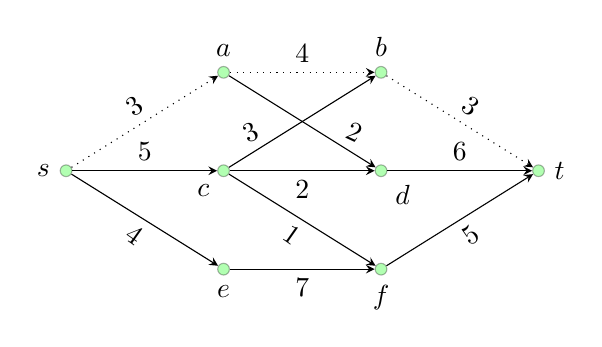
\begin{tikzpicture}
                    \node[circle, draw, inner sep=1.5pt, fill=green, opacity=0.3, label={-180:$s$}] (s) at (0, 0) {};
                    \node[circle, draw, inner sep=1.5pt, fill=green, opacity=0.3, label={90:$a$}] (a) at (2, 1.25) {};
                    \node[circle, draw, inner sep=1.5pt, fill=green, opacity=0.3, label={90:$b$}] (b) at (4, 1.25) {};
                    \node[circle, draw, inner sep=1.5pt, fill=green, opacity=0.3, label={-135:$c$}] (c) at (2, 0) {};
                    \node[circle, draw, inner sep=1.5pt, fill=green, opacity=0.3, label={-45:$d$}] (d) at (4, 0) {};
                    \node[circle, draw, inner sep=1.5pt, fill=green, opacity=0.3, label={-90:$e$}] (e) at (2, -1.25) {};
                    \node[circle, draw, inner sep=1.5pt, fill=green, opacity=0.3, label={-90:$f$}] (f) at (4, -1.25) {};
                    \node[circle, draw, inner sep=1.5pt, fill=green, opacity=0.3, label={0:$t$}] (t) at (6, 0) {};

                    \draw[-stealth, dotted] (s) -- node[above, rotate=35] {$3$} (a);
                    \draw[-stealth] (s) -- node[above] {$5$} (c);
                    \draw[-stealth] (s) -- node[below, rotate=-35] {$4$} (e);
                    \draw[-stealth, dotted] (a) -- node[above] {$4$} (b);
                    \draw[-stealth] (e) -- node[below] {$7$} (f);
                    \draw[-stealth, dotted] (b) -- node[above, rotate=-35] {$3$} (t);
                    \draw[-stealth] (d) -- node[above] {$6$} (t);
                    \draw[-stealth] (f) -- node[below, rotate=35] {$5$} (t);
                    \draw[-stealth] (c) -- node[below] {$2$} (d);
                    \draw[-stealth] (a) -- node[above, rotate=-25, pos=0.8] {$2$} (d);
                    \draw[-stealth] (c) -- node[above, rotate=25, pos=0.2] {$3$} (b);
                    \draw[-stealth] (c) -- node[below, rotate=-35] {$1$} (f);
                \end{tikzpicture}
            }
        \end{subfigure}
    \end{figure}
    \noindent Note that at the start, the residual graph only has forwards-edges of full capacity- the flow is 0, so we have no backwards edge, and we just have a forwards edge equal to the slack. The dotted path on the right shows the (shortest) path on the residual graph. This is an augmenting path in the network, which we use to increase the flow to 3.
    \begin{figure}[H]
        \centering
        \begin{subfigure}{0.48\textwidth}
            \centering
            \scalebox{0.8}{
                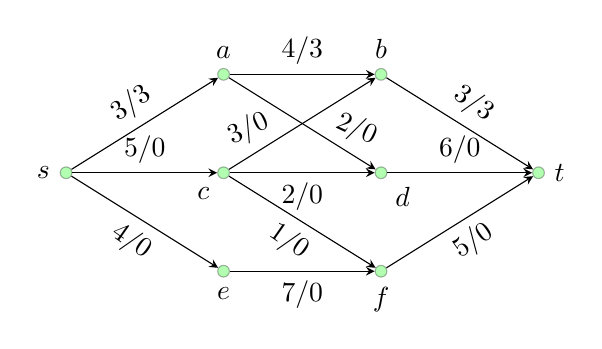
\begin{tikzpicture}
                    \node[circle, draw, inner sep=1.5pt, fill=green, opacity=0.3, label={-180:$s$}] (s) at (0, 0) {};
                    \node[circle, draw, inner sep=1.5pt, fill=green, opacity=0.3, label={90:$a$}] (a) at (2, 1.25) {};
                    \node[circle, draw, inner sep=1.5pt, fill=green, opacity=0.3, label={90:$b$}] (b) at (4, 1.25) {};
                    \node[circle, draw, inner sep=1.5pt, fill=green, opacity=0.3, label={-135:$c$}] (c) at (2, 0) {};
                    \node[circle, draw, inner sep=1.5pt, fill=green, opacity=0.3, label={-45:$d$}] (d) at (4, 0) {};
                    \node[circle, draw, inner sep=1.5pt, fill=green, opacity=0.3, label={-90:$e$}] (e) at (2, -1.25) {};
                    \node[circle, draw, inner sep=1.5pt, fill=green, opacity=0.3, label={-90:$f$}] (f) at (4, -1.25) {};
                    \node[circle, draw, inner sep=1.5pt, fill=green, opacity=0.3, label={0:$t$}] (t) at (6, 0) {};

                    \draw[-stealth] (s) -- node[above, rotate=35] {$3/3$} (a);
                    \draw[-stealth] (s) -- node[above] {$5/0$} (c);
                    \draw[-stealth] (s) -- node[below, rotate=-35] {$4/0$} (e);
                    \draw[-stealth] (a) -- node[above] {$4/3$} (b);
                    \draw[-stealth] (e) -- node[below] {$7/0$} (f);
                    \draw[-stealth] (b) -- node[above, rotate=-35] {$3/3$} (t);
                    \draw[-stealth] (d) -- node[above] {$6/0$} (t);
                    \draw[-stealth] (f) -- node[below, rotate=35] {$5/0$} (t);
                    \draw[-stealth] (c) -- node[below] {$2/0$} (d);
                    \draw[-stealth] (a) -- node[above, rotate=-25, pos=0.8] {$2/0$} (d);
                    \draw[-stealth] (c) -- node[above, rotate=25, pos=0.2] {$3/0$} (b);
                    \draw[-stealth] (c) -- node[below, rotate=-35] {$1/0$} (f);
                \end{tikzpicture}
            }
        \end{subfigure}
        \hfill
        \begin{subfigure}{0.48\textwidth}
            \centering
            \scalebox{0.8}{
                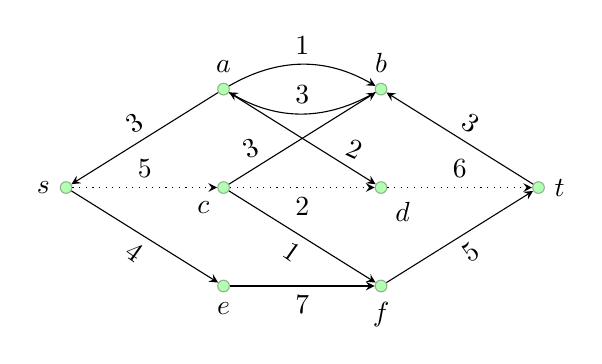
\begin{tikzpicture}
                    \node[circle, draw, inner sep=1.5pt, fill=green, opacity=0.3, label={-180:$s$}] (s) at (0, 0) {};
                    \node[circle, draw, inner sep=1.5pt, fill=green, opacity=0.3, label={90:$a$}] (a) at (2, 1.25) {};
                    \node[circle, draw, inner sep=1.5pt, fill=green, opacity=0.3, label={90:$b$}] (b) at (4, 1.25) {};
                    \node[circle, draw, inner sep=1.5pt, fill=green, opacity=0.3, label={-135:$c$}] (c) at (2, 0) {};
                    \node[circle, draw, inner sep=1.5pt, fill=green, opacity=0.3, label={-45:$d$}] (d) at (4, 0) {};
                    \node[circle, draw, inner sep=1.5pt, fill=green, opacity=0.3, label={-90:$e$}] (e) at (2, -1.25) {};
                    \node[circle, draw, inner sep=1.5pt, fill=green, opacity=0.3, label={-90:$f$}] (f) at (4, -1.25) {};
                    \node[circle, draw, inner sep=1.5pt, fill=green, opacity=0.3, label={0:$t$}] (t) at (6, 0) {};

                    \draw[-stealth] (a) -- node[above, rotate=35] {$3$} (s);
                    \draw[-stealth, dotted] (s) -- node[above] {$5$} (c);
                    \draw[-stealth] (s) -- node[below, rotate=-35] {$4$} (e);
                    \draw[-stealth] (a) edge[bend left] node[above] {$1$} (b);
                    \draw[-stealth] (b) edge[bend left] node[above] {$3$} (a);
                    \draw[-stealth] (e) -- node[below] {$7$} (f);
                    \draw[-stealth] (t) -- node[above, rotate=-35] {$3$} (b);
                    \draw[-stealth, dotted] (d) -- node[above] {$6$} (t);
                    \draw[-stealth] (f) -- node[below, rotate=35] {$5$} (t);
                    \draw[-stealth, dotted] (c) -- node[below] {$2$} (d);
                    \draw[-stealth] (a) -- node[above, rotate=-25, pos=0.8] {$2$} (d);
                    \draw[-stealth] (c) -- node[above, rotate=25, pos=0.2] {$3$} (b);
                    \draw[-stealth] (c) -- node[below, rotate=-35] {$1$} (f);
                \end{tikzpicture}
            }
        \end{subfigure}
    \end{figure}
    \noindent Typically, when the flow changes, we do not need to re-construct the residual graph; we just modify some edge weights. In this case, the edge $(a, b)$ has its weight reduced to 1, $(s, a)$ flips to $(a, s)$ and so on. We now take the next path in the residue, and augment the network flow using it:
    \begin{figure}[H]
        \centering
        \begin{subfigure}{0.48\textwidth}
            \centering
            \scalebox{0.8}{
                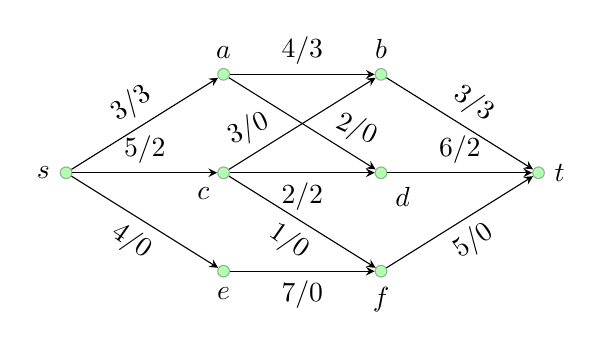
\begin{tikzpicture}
                    \node[circle, draw, inner sep=1.5pt, fill=green, opacity=0.3, label={-180:$s$}] (s) at (0, 0) {};
                    \node[circle, draw, inner sep=1.5pt, fill=green, opacity=0.3, label={90:$a$}] (a) at (2, 1.25) {};
                    \node[circle, draw, inner sep=1.5pt, fill=green, opacity=0.3, label={90:$b$}] (b) at (4, 1.25) {};
                    \node[circle, draw, inner sep=1.5pt, fill=green, opacity=0.3, label={-135:$c$}] (c) at (2, 0) {};
                    \node[circle, draw, inner sep=1.5pt, fill=green, opacity=0.3, label={-45:$d$}] (d) at (4, 0) {};
                    \node[circle, draw, inner sep=1.5pt, fill=green, opacity=0.3, label={-90:$e$}] (e) at (2, -1.25) {};
                    \node[circle, draw, inner sep=1.5pt, fill=green, opacity=0.3, label={-90:$f$}] (f) at (4, -1.25) {};
                    \node[circle, draw, inner sep=1.5pt, fill=green, opacity=0.3, label={0:$t$}] (t) at (6, 0) {};

                    \draw[-stealth] (s) -- node[above, rotate=35] {$3/3$} (a);
                    \draw[-stealth] (s) -- node[above] {$5/2$} (c);
                    \draw[-stealth] (s) -- node[below, rotate=-35] {$4/0$} (e);
                    \draw[-stealth] (a) -- node[above] {$4/3$} (b);
                    \draw[-stealth] (e) -- node[below] {$7/0$} (f);
                    \draw[-stealth] (b) -- node[above, rotate=-35] {$3/3$} (t);
                    \draw[-stealth] (d) -- node[above] {$6/2$} (t);
                    \draw[-stealth] (f) -- node[below, rotate=35] {$5/0$} (t);
                    \draw[-stealth] (c) -- node[below] {$2/2$} (d);
                    \draw[-stealth] (a) -- node[above, rotate=-25, pos=0.8] {$2/0$} (d);
                    \draw[-stealth] (c) -- node[above, rotate=25, pos=0.2] {$3/0$} (b);
                    \draw[-stealth] (c) -- node[below, rotate=-35] {$1/0$} (f);
                \end{tikzpicture}
            }
        \end{subfigure}
        \hfill
        \begin{subfigure}{0.48\textwidth}
            \centering
            \scalebox{0.8}{
                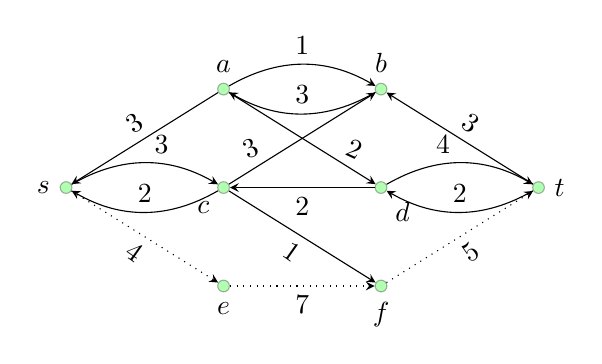
\begin{tikzpicture}
                    \node[circle, draw, inner sep=1.5pt, fill=green, opacity=0.3, label={-180:$s$}] (s) at (0, 0) {};
                    \node[circle, draw, inner sep=1.5pt, fill=green, opacity=0.3, label={90:$a$}] (a) at (2, 1.25) {};
                    \node[circle, draw, inner sep=1.5pt, fill=green, opacity=0.3, label={90:$b$}] (b) at (4, 1.25) {};
                    \node[circle, draw, inner sep=1.5pt, fill=green, opacity=0.3, label={-135:$c$}] (c) at (2, 0) {};
                    \node[circle, draw, inner sep=1.5pt, fill=green, opacity=0.3, label={-45:$d$}] (d) at (4, 0) {};
                    \node[circle, draw, inner sep=1.5pt, fill=green, opacity=0.3, label={-90:$e$}] (e) at (2, -1.25) {};
                    \node[circle, draw, inner sep=1.5pt, fill=green, opacity=0.3, label={-90:$f$}] (f) at (4, -1.25) {};
                    \node[circle, draw, inner sep=1.5pt, fill=green, opacity=0.3, label={0:$t$}] (t) at (6, 0) {};

                    \draw[-stealth] (a) -- node[above, rotate=35] {$3$} (s);
                    \draw[-stealth] (s) edge[bend left] node[above right] {$3$} (c);
                    \draw[-stealth] (c) edge[bend left] node[above] {$2$} (s);
                    \draw[-stealth, dotted] (s) -- node[below, rotate=-35] {$4$} (e);
                    \draw[-stealth] (a) edge[bend left] node[above] {$1$} (b);
                    \draw[-stealth] (b) edge[bend left] node[above] {$3$} (a);
                    \draw[-stealth, dotted] (e) -- node[below] {$7$} (f);
                    \draw[-stealth] (t) -- node[above, rotate=-35] {$3$} (b);
                    \draw[-stealth] (d) edge[bend left] node[above left] {$4$} (t);
                    \draw[-stealth] (t) edge[bend left] node[above] {$2$} (d);
                    \draw[-stealth, dotted] (f) -- node[below, rotate=35] {$5$} (t);
                    \draw[-stealth] (d) -- node[below] {$2$} (c);
                    \draw[-stealth] (a) -- node[above, rotate=-25, pos=0.8] {$2$} (d);
                    \draw[-stealth] (c) -- node[above, rotate=25, pos=0.2] {$3$} (b);
                    \draw[-stealth] (c) -- node[below, rotate=-35] {$1$} (f);
                \end{tikzpicture}
            }
        \end{subfigure}
    \end{figure}
    \noindent We have now increased the network flow value to 5. Using the dotted path (and further paths in the iteration), we can continue improving the capacity of the network until we get the following state:    
    \begin{figure}[H]
        \centering
        \begin{subfigure}{0.48\textwidth}
            \centering
            \scalebox{0.8}{
                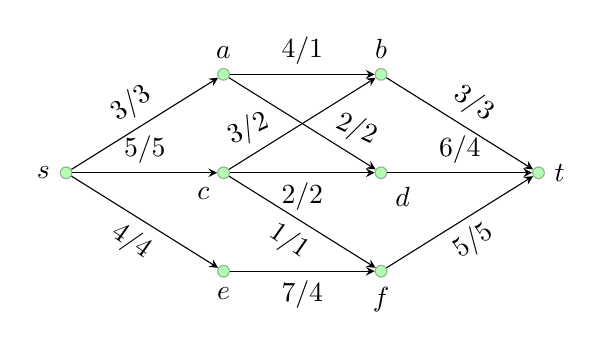
\begin{tikzpicture}
                    \node[circle, draw, inner sep=1.5pt, fill=green, opacity=0.3, label={-180:$s$}] (s) at (0, 0) {};
                    \node[circle, draw, inner sep=1.5pt, fill=green, opacity=0.3, label={90:$a$}] (a) at (2, 1.25) {};
                    \node[circle, draw, inner sep=1.5pt, fill=green, opacity=0.3, label={90:$b$}] (b) at (4, 1.25) {};
                    \node[circle, draw, inner sep=1.5pt, fill=green, opacity=0.3, label={-135:$c$}] (c) at (2, 0) {};
                    \node[circle, draw, inner sep=1.5pt, fill=green, opacity=0.3, label={-45:$d$}] (d) at (4, 0) {};
                    \node[circle, draw, inner sep=1.5pt, fill=green, opacity=0.3, label={-90:$e$}] (e) at (2, -1.25) {};
                    \node[circle, draw, inner sep=1.5pt, fill=green, opacity=0.3, label={-90:$f$}] (f) at (4, -1.25) {};
                    \node[circle, draw, inner sep=1.5pt, fill=green, opacity=0.3, label={0:$t$}] (t) at (6, 0) {};

                    \draw[-stealth] (s) -- node[above, rotate=35] {$3/3$} (a);
                    \draw[-stealth] (s) -- node[above] {$5/5$} (c);
                    \draw[-stealth] (s) -- node[below, rotate=-35] {$4/4$} (e);
                    \draw[-stealth] (a) -- node[above] {$4/1$} (b);
                    \draw[-stealth] (e) -- node[below] {$7/4$} (f);
                    \draw[-stealth] (b) -- node[above, rotate=-35] {$3/3$} (t);
                    \draw[-stealth] (d) -- node[above] {$6/4$} (t);
                    \draw[-stealth] (f) -- node[below, rotate=35] {$5/5$} (t);
                    \draw[-stealth] (c) -- node[below] {$2/2$} (d);
                    \draw[-stealth] (a) -- node[above, rotate=-25, pos=0.8] {$2/2$} (d);
                    \draw[-stealth] (c) -- node[above, rotate=25, pos=0.2] {$3/2$} (b);
                    \draw[-stealth] (c) -- node[below, rotate=-35] {$1/1$} (f);
                \end{tikzpicture}
            }
        \end{subfigure}
        \hfill
        \begin{subfigure}{0.48\textwidth}
            \centering
            \scalebox{0.8}{
                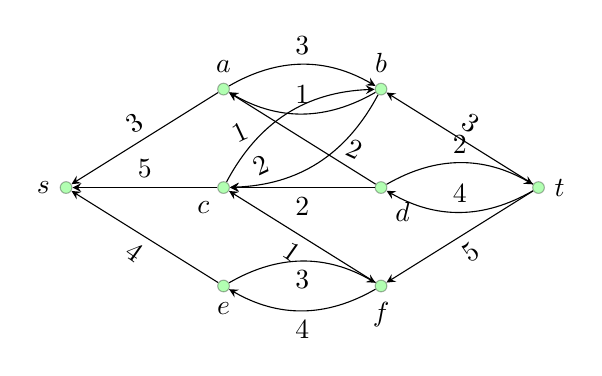
\begin{tikzpicture}
                    \node[circle, draw, inner sep=1.5pt, fill=green, opacity=0.3, label={-180:$s$}] (s) at (0, 0) {};
                    \node[circle, draw, inner sep=1.5pt, fill=green, opacity=0.3, label={90:$a$}] (a) at (2, 1.25) {};
                    \node[circle, draw, inner sep=1.5pt, fill=green, opacity=0.3, label={90:$b$}] (b) at (4, 1.25) {};
                    \node[circle, draw, inner sep=1.5pt, fill=green, opacity=0.3, label={-135:$c$}] (c) at (2, 0) {};
                    \node[circle, draw, inner sep=1.5pt, fill=green, opacity=0.3, label={-45:$d$}] (d) at (4, 0) {};
                    \node[circle, draw, inner sep=1.5pt, fill=green, opacity=0.3, label={-90:$e$}] (e) at (2, -1.25) {};
                    \node[circle, draw, inner sep=1.5pt, fill=green, opacity=0.3, label={-90:$f$}] (f) at (4, -1.25) {};
                    \node[circle, draw, inner sep=1.5pt, fill=green, opacity=0.3, label={0:$t$}] (t) at (6, 0) {};

                    \draw[-stealth] (a) -- node[above, rotate=35] {$3$} (s);
                    \draw[-stealth] (c) -- node[above] {$5$} (s);
                    \draw[-stealth] (e) -- node[below, rotate=-35] {$4$} (s);
                    \draw[-stealth] (a) edge[bend left] node[above] {$3$} (b);
                    \draw[-stealth] (b) edge[bend left] node[above] {$1$} (a);
                    \draw[-stealth] (e) edge[bend left] node[below] {$3$} (f);
                    \draw[-stealth] (f) edge[bend left] node[below] {$4$} (e);
                    \draw[-stealth] (t) -- node[above, rotate=-35] {$3$} (b);
                    \draw[-stealth] (d) edge[bend left] node[above] {$2$} (t);
                    \draw[-stealth] (t) edge[bend left] node[above] {$4$} (d);
                    \draw[-stealth] (t) -- node[below, rotate=35] {$5$} (f);
                    \draw[-stealth] (d) -- node[below] {$2$} (c);
                    \draw[-stealth] (d) -- node[above, rotate=-25, pos=0.2] {$2$} (a);
                    \draw[-stealth] (c) edge[bend left] node[above, rotate=25, pos=0.2] {$1$} (b);
                    \draw[-stealth] (b) edge[bend left] node[above, rotate=25, pos=0.8] {$2$} (c);
                    \draw[-stealth] (f) -- node[below, rotate=-35] {$1$} (c);
                \end{tikzpicture}
            }
        \end{subfigure}
    \end{figure}
    \noindent In the residue graph, the source $s$ has become a sink. Hence, we cannot find a path from the source to the sink $t$. We have found the maximum flow- it has value 12. If we constructed the cut corresponding to this maximum flow, we would find $A = \{s\}$ and $B = \{a, b, c, d, e, f, t\}$. The generated cut is $C = \{(s, a), (s, c), (s, e)\}$, which has value 12. Hence, the Max-Flow Min-Cut theorem tells us that it is a maximum flow.

    We can convert an instance of maximum-cardinality matching to a network flow instance. Let the vertex set be partitioned into left vertices $L$ and right vertices $R$. For every edge $\{u, v\}$, if $u \in L$ and $v \in R$, then the network has a directed edge $(u, v)$. We also have a source $s$, which has edges to every vertex in $L$, and a sink $t$, which has edges from every vertex in $R$. The capacity of each edge in the network is 1. For example, consider the two figures below:
    \begin{figure}[H]
        \centering
        \begin{subfigure}{0.45\textwidth}
            \centering
            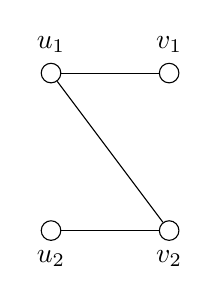
\begin{tikzpicture}
                \node[circle, draw, inner sep=2.5pt, label={90:$u_1$}] (u1) at (0, 0) {};
                \node[circle, draw, inner sep=2.5pt, label={90:$v_1$}] (v1) at (1.5, 0) {};
                \node[circle, draw, inner sep=2.5pt, label={-90:$u_2$}] (u2) at (0, -2) {};
                \node[circle, draw, inner sep=2.5pt, label={-90:$v_2$}] (v2) at (1.5, -2) {};

                \draw (u1) -- (v1);
                \draw (u1) -- (v2);
                \draw (u2) -- (v2);
            \end{tikzpicture}
        \end{subfigure}
        \hfill
        \begin{subfigure}{0.45\textwidth}
            \centering
            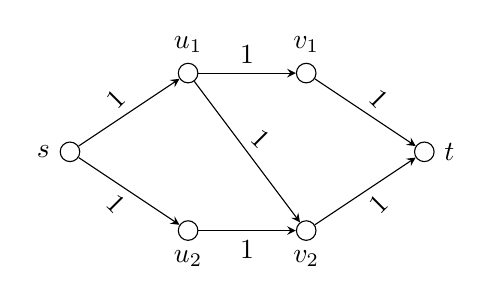
\begin{tikzpicture}
                \node[circle, draw, inner sep=2.5pt, label={180:$s$}] (s) at (-1.5, -1) {};
                \node[circle, draw, inner sep=2.5pt, label={90:$u_1$}] (u1) at (0, 0) {};
                \node[circle, draw, inner sep=2.5pt, label={90:$v_1$}] (v1) at (1.5, 0) {};
                \node[circle, draw, inner sep=2.5pt, label={-90:$u_2$}] (u2) at (0, -2) {};
                \node[circle, draw, inner sep=2.5pt, label={-90:$v_2$}] (v2) at (1.5, -2) {};
                \node[circle, draw, inner sep=2.5pt, label={0:$t$}] (t) at (3, -1) {};

                \draw[-stealth] (s) -- node[above, rotate=45] {1} (u1);
                \draw[-stealth] (s) -- node[below, rotate=-45] {1} (u2);
                \draw[-stealth] (u1) -- node[above] {1} (v1);
                \draw[-stealth] (u1) -- node[above, rotate=-45] {1} (v2);
                \draw[-stealth] (u2) -- node[below] {1} (v2);
                \draw[-stealth] (v1) -- node[above, rotate=-45] {1} (t);
                \draw[-stealth] (v2) -- node[below, rotate=45] {1} (t);
            \end{tikzpicture}
        \end{subfigure}
    \end{figure}
    \noindent On the left, we have an instance of maximum cardinality matching. Its equivalent instance is given on the right- the directed version of the edges present, along with the source $s$ and the sink $t$. Using the network flow algorithm, we will get the the same result. We illustrate this for the example above below:
    \begin{figure}[H]
        \centering
        \begin{subfigure}{0.45\textwidth}
            \centering
            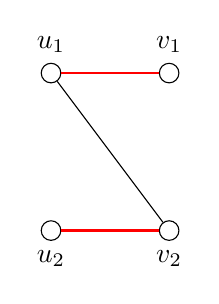
\begin{tikzpicture}
                \node[circle, draw, inner sep=2.5pt, label={90:$u_1$}] (u1) at (0, 0) {};
                \node[circle, draw, inner sep=2.5pt, label={90:$v_1$}] (v1) at (1.5, 0) {};
                \node[circle, draw, inner sep=2.5pt, label={-90:$u_2$}] (u2) at (0, -2) {};
                \node[circle, draw, inner sep=2.5pt, label={-90:$v_2$}] (v2) at (1.5, -2) {};

                \draw[red, thick] (u1) -- (v1);
                \draw (u1) -- (v2);
                \draw[red, thick] (u2) -- (v2);
            \end{tikzpicture}
        \end{subfigure}
        \hfill
        \begin{subfigure}{0.45\textwidth}
            \centering
            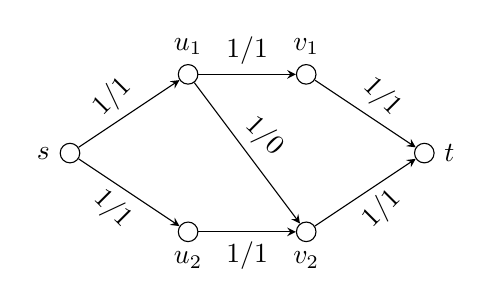
\begin{tikzpicture}
                \node[circle, draw, inner sep=2.5pt, label={180:$s$}] (s) at (-1.5, -1) {};
                \node[circle, draw, inner sep=2.5pt, label={90:$u_1$}] (u1) at (0, 0) {};
                \node[circle, draw, inner sep=2.5pt, label={90:$v_1$}] (v1) at (1.5, 0) {};
                \node[circle, draw, inner sep=2.5pt, label={-90:$u_2$}] (u2) at (0, -2) {};
                \node[circle, draw, inner sep=2.5pt, label={-90:$v_2$}] (v2) at (1.5, -2) {};
                \node[circle, draw, inner sep=2.5pt, label={0:$t$}] (t) at (3, -1) {};

                \draw[-stealth] (s) -- node[above, rotate=45] {1/1} (u1);
                \draw[-stealth] (s) -- node[below, rotate=-45] {1/1} (u2);
                \draw[-stealth] (u1) -- node[above] {1/1} (v1);
                \draw[-stealth] (u1) -- node[above, rotate=-45] {1/0} (v2);
                \draw[-stealth] (u2) -- node[below] {1/1} (v2);
                \draw[-stealth] (v1) -- node[above, rotate=-45] {1/1} (t);
                \draw[-stealth] (v2) -- node[below, rotate=45] {1/1} (t);
            \end{tikzpicture}
        \end{subfigure}
    \end{figure}
    \noindent The edges $\{u_1, v_1\}$ and $\{u_2, v_2\}$ are part of the maximum cardinality matching, as seen on the left. This can be inferred from right too- these edges are precisely those with flow value 1. If we use the network flow version of the algorithm, we will get a more efficient algorithm- it is $O(\sqrt{|V|}(|V| + |E|))$ instead of $O(|V| (|V| + |E|))$ we saw above.


\end{document}